\input{../style/preamble}
\input{../latex-math/basic-math}
\input{../latex-math/basic-ml}
\input{../latex-math/ml-nn}

\newcommand{\titlefigure}{figure/backprop_gg_new.png}
\newcommand{\learninggoals}{
  \item Computational graphs and the chain rule as the mathematical basis of backpropagation
  \item The forward and backward pass, worked through a concrete example
  \item General backpropagation formalism via recursive application of the chain rule
  \item Why and how to initialize network weights and biases
  \item Optimization challenges in deep networks: ill-conditioning, local minima, saddle points, cliffs/exploding gradients
}

\title{Advanced Artificial Intelligence and Machine Learning}
\date{}

\begin{document}

\lecturechapter{Backpropagation}
\lecture{Advanced AI \& ML}
%%%%%%%%%%%%%%%%%%%%%%%%%%%%%%%%%%%%%%%%%%%%%%%%%%%%%%%%%%%%%%%%%%
\section{Chain Rule and Computational Graphs}

%%%%%%%%%%%%%%%%%%%%%%%%%%%%%%%%%%%%%%%%%%%%%%%%%%%%%%%%%%%%%%%%%%

%\begin{frame}
%\frametitle{Lecture outline}
%\tableofcontents
%\end{frame}
%%%%%%%%%%%%%%%%%%%%%%%%%%%%%%%%%%%%%%%%%%%%%%%%%%%%%%%%%%%%%%%%%%
% \begin{frame}{Local Minima/Convexity}
% \end{frame}

% \section{Chain Rule and Computational Graphs}
%%%%%%%%%%%%%%%%%%%%%%%%%%%%%%%%%%%%%%%%%%%%%%%%%%%%%%%%%%%%%%%%%%
\begin{vbframe}{Chain rule of calculus}
  % \begin{itemize}
  %   \item The chain rule can be used to compute derivatives of the composition of two or more functions.
  %   \item Let $x \in \R^m$, $y \in \R^n$, \\
  %         $g: \R^m \to \R^n$ and $f: \R^n \to \R$. \\
  %   \item If $y = g(x)$ and $z = f(y)$, the chain rule yields $$\frac{\partial z}{\partial x_i} = \sum_j \frac{\partial z}{\partial y_j} \frac{\partial y_j}{\partial x_i}$$
  %         or in vector notation $$\nabla_x z = \Big(\frac{\partial y}{\partial x}\Big)^\top \nabla_y z,$$
  %         where $\frac{\partial y}{\partial x}$ is the $n \times m$ jacobian matrix of $g$.
  % \end{itemize}
  \begin{itemize}
    \item The chain rule can be used to compute derivatives of the composition of two or more functions.
    \item Let $\xv \in \R^m$, $\mathbf{y} \in \R^n$, \\
          $g: \R^m \to \R^n$ and $f: \R^n \to \R$. \\
    \item If $\mathbf{y} = g(\xv)$ and $z = f(\mathbf{y})$, the chain rule yields: $$\frac{\partial z}{\partial x_i} = \sum_j \frac{\partial z}{\partial y_j} \cdot \frac{\partial y_j}{\partial x_i}$$
          or, in vector notation: $$\nabla_{\xv} z = \Big(\frac{\partial \mathbf{y}}{\partial \xv}\Big)^\top \nabla_{\mathbf{y}} z,$$
          where $\frac{\partial \mathbf{y}}{\partial \xv}$ is the ($n \times m$) Jacobian matrix of $g$.
  \end{itemize}
\end{vbframe}  

\begin{vbframe}{Computational graphs}
  \begin{minipage}{0.5\textwidth}
    \begin{itemize}
      \item CGs are nested expresssions, visualized as graphs.
      \item Each node is a variable, either an input or derived.
      \item Derived variables are functions applied to other variables.
    \end{itemize}
  \end{minipage}\hfill
  \begin{minipage}{0.5\textwidth}
    \begin{figure}
      \centering
        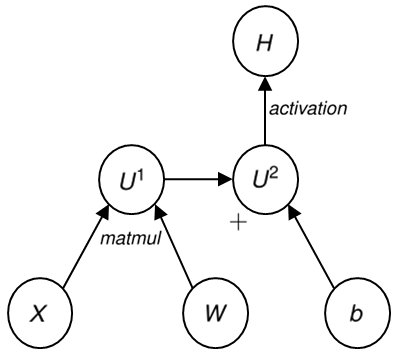
\includegraphics[width=6cm]{figure/compgraph1.png}
        \tiny{\\source : Goodfellow et al. (2016)}
        \caption{The computational graph for the expression $H = \sigma(XW + B)$ with activation function $\sigma(\cdot)$.}
    \end{figure}
  \end{minipage}  
\end{vbframe}

\begin{vbframe}{Chain rule of calculus: Example 1}
  \begin{minipage}{0.5\textwidth}
    \begin{itemize}
      \item Suppose we have the following computational graph.
      \item To compute the derivative of $\frac{\partial z}{\partial w}$ %$\frac{\partial z}{\partial w}$ 
      we need to recursively apply the chain rule. That is:
      \begin{eqnarray*}
        \frac{\partial z}{\partial w} &=& \frac{\partial z}{\partial y} \cdot \frac{\partial y}{\partial x} \cdot \frac{\partial x}{\partial w} \\
                                  &=& f'_3(y) \cdot f'_2(x) \cdot f'_1(w) \\
                                  &=& f'_3(f_2(f_1(w))) \cdot f'_2(f_1(w)) \cdot f'_1(w)
      \end{eqnarray*}
    \end{itemize}
  \end{minipage}\hfill
  \begin{minipage}{0.32\textwidth}
    \begin{figure}
      \centering
        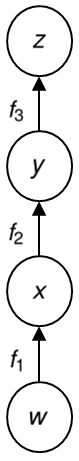
\includegraphics[width=1cm]{figure/compgraph2.png}
        \begin{footnotesize}
        \tiny{\\source : Goodfellow et al. (2016)}
        \caption{A computational graph, such that $x = f_1(w),$ $y = f_2(x)$ and $z = f_3(y)$.}
        \end{footnotesize}
    \end{figure}
  \end{minipage}
% \framebreak
%   \begin{figure}
%     \centering
%       \includegraphics[width=4.5cm]{figure/compgraph3.png}
%       \caption{Applying the chain rule to the example yields us a computational graph with a symbolic description of the
% derivatives.}
%   \end{figure}  
\end{vbframe}

\begin{frame}{Chain rule of calculus: Example 2}
  \small

   \begin{figure}
    \centering
      \scalebox{0.22}{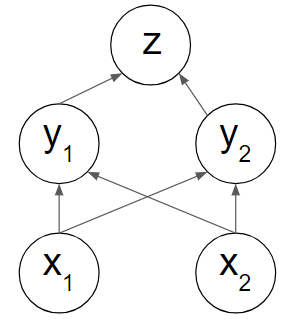
\includegraphics{figure/chain_tree.png}}
  \end{figure}

To compute $\nabla_\xv z$, we apply the chain rule % to the computational graph above,
  \begin{itemize}
    \setlength{\itemsep}{1pt}
    \item $\frac {\partial z}{\partial x_1} = \sum_j \frac{\partial z}{\partial y_j} \frac{\partial y_j}{\partial x_1} = \frac {\partial z}{\partial y_1} \frac {\partial y_1}{\partial x_1} + \frac {\partial z}{\partial y_2} \frac {\partial y_2}{\partial x_1}$
    \item $\frac {\partial z}{\partial x_2} = \sum_j \frac{\partial z}{\partial y_j} \frac{\partial y_j}{\partial x_2} = \frac {\partial z}{\partial y_1} \frac {\partial y_1}{\partial x_2} + \frac {\partial z}{\partial y_2} \frac {\partial y_2}{\partial x_2}$
  \end{itemize}
  \vspace{1mm}
    Therefore, the gradient of $z$ w.r.t $\xv$ is
    \begin{itemize}
      \item  $\nabla_\xv z = \begin{bmatrix}
               \frac {\partial z}{\partial x_1} \\
               \frac {\partial z}{\partial x_2} \\
             \end{bmatrix} = \underbrace{\begin{bmatrix} \frac{\partial y_1}{\partial x_1}&\frac {\partial y_2}{\partial x_1}\\
                                             \frac {\partial y_1}{\partial x_2}&\frac {\partial y_2}{\partial x_2}\\
             \end{bmatrix}}_{\textcolor{red}{(\frac{\partial \mathbf{y}}{\partial \xv})^\top}} \underbrace{\begin{bmatrix} \frac {\partial z}{\partial y_1} \\
            \frac {\partial z}{\partial y_2} \\ \end{bmatrix}}_{\textcolor{red}{\nabla_{\mathbf{y}} z}} = \Big(\frac{\partial \mathbf{y}}{\partial \xv}\Big)^\top \nabla_{\mathbf{y}} z $
  \end{itemize}
\end{frame}

\begin{frame} {Computational Graph: Neural Net}
  \begin{figure}
      \centering
        \scalebox{0.55}{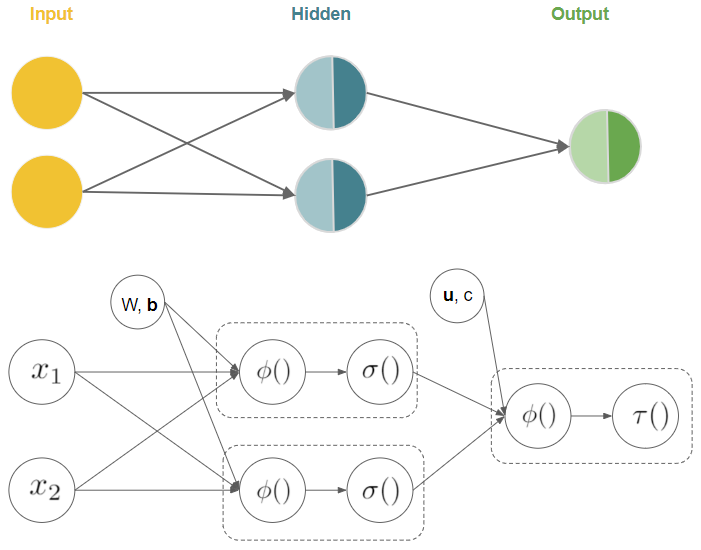
\includegraphics{figure/neo_comp.png}}
        \caption{\footnotesize A neural network can be seen as a computational graph. $\phi$ is the weighted sum and $\sigma$ and $\tau$ are the activations. \\
        Note: In contrast to the top figure, the arrows in the computational graph below merely indicate \textbf{dependence}, not weights.}
    \end{figure}
\end{frame}
% \begin{frame}{Chain rule of calculus}
% \begin{figure}
%     \centering
%       \scalebox{0.4}{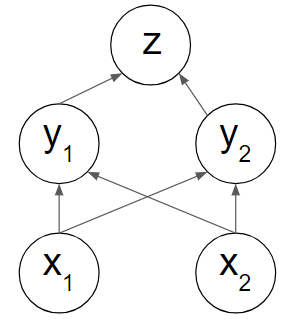
\includegraphics{figure/chain_tree.png}}
%   \end{figure}
%   
%     $\nabla_x z = \begin{bmatrix}
%            \frac {\partial z}{\partial x_1} \\
%            \frac {\partial z}{\partial x_2} \\
%          \end{bmatrix} = \begin{bmatrix}
%            \frac {\partial z}{\partial x_1} \\
%            \frac {\partial z}{\partial x_2} \\
%          \end{bmatrix}$
% \end{frame}


%%%%%%%%%%%%%%%%%%%%%%%%%%%%%%%%%%%%%%%%%%%%%%%%%%%%%%%%%%%%%%%%%%
%%%%%%%%%%%%%%%%%%%%%%%%%%%%%%%%%%%%%%%%%%%%%%%%%%%%%%%%%%%%%%%%%%
% \begin{frame} {Simple Example?}
%   \begin{figure}
%     \centering
%       \scalebox{1}{\includegraphics{figure/simex.png}}
%   \end{figure}
% \end{frame}
%%%%%%%%%%%%%%%%%%%%%%%%%%%%%%%%%%%%%%%%%%%%%%%%%%%%%%%%%%%%%%%%%%

%%%%%%%%%%%%%%%%%%%%%%%%%%%%%%%%%%%%%%%%%%%%%%%%%%%%%%%%%%%%%%%%%%
%%%%%%%%%%%%%%%%%%%%%%%%%%%%%%%%%%%%%%%%%%%%%%%%%%%%%%%%%%%%%%%%%%
%%%%%%%%%%%%%%%%%%          REFERENCES          %%%%%%%%%%%%%%%%%%
%%%%%%%%%%%%%%%%%%%%%%%%%%%%%%%%%%%%%%%%%%%%%%%%%%%%%%%%%%%%%%%%%%

%\section{References}

%\begin{vbframe}
%\frametitle{References}
%\footnotesize{
%\begin{thebibliography}{99}

%%%%%%%%%%%%%%%%%%%%%%%%%%%%%%%%%%%
%\bibitem[Ian Goodfellow et al., 2016]{1} Ian Goodfellow, Yoshua Bengio and Aaron Courville (2016)
%\newblock Deep Learning
%\newblock \emph{\url{http://www.deeplearningbook.org/}}
%%%%%%%%%%%%%%%%%%%%%%%%%%%%%%%%%%%

%\end{thebibliography}
%}
%\end{vbframe}
%%%%%%%%%%%%%%%%%%%%%%%%%%%%%%%%%%%%%%%%%%%%%%%%%%%%%%%%%%%%%%%%%%
%%%%%%%%%%%%%%%%%%%%%%%%%%%%%%%%%%%%%%%%%%%%%%%%%%%%%%%%%%%%%%%%%%


\section{Basic Backpropagation 1}
%%%%%%%%%%%%%%%%%%%%%%%%%%%%%%%%%%%%%%%%%%%%%%%%%%%%%%%%%%%%%%%%%%

\begin{frame}{Backpropagation: Basic Idea}
We would like to run ERM by GD on: $$ \risket = \frac{1}{n} \sumin \Lxyit$$ 
% where $\thetav$ are the weights (and biases) of the network. 

Backprop training of NNs runs in 2 alternating steps, for one $\xv$:
\begin{enumerate}
\item \textbf{Forward pass:} Inputs flow through model to outputs. 
    We then compute the observation loss. We covered that.
\item \textbf{Backward pass:} Loss flows backwards to update weights so error is reduced,
    as in GD.
\end{enumerate}
\lz
We will see: This is simply (S)GD in disguise, cleverly using the chain rule, so we can reuse
a lot of intermediate results.
\end{frame}
%%%%%%%%%%%%%%%%%%%%%%%%%%%%%%%%%%%%%%%%%%%%%%%%%%%%%%%%%%%%%%%%%%

% \begin{vbframe}{Weight update rule}
  % \begin{itemize}
    % \item Backpropagation can then be used to compute the gradient of $\Lxyt$ in an \textbf{extremely} efficient way.
    % \item  In GD, the weight for one $\xv$ with learning rate $\alpha$, is 
      % $$\thetav^{[t+1]} = \thetav^{[t]} - \alpha \cdot \nabla_{\theta}L\left(y, f\left(\xv ~|~ \thetav^{[t]}\right)\right)$$ 
        % \item We will see that, at its core, backpropagation is just a clever implementation of the chain rule. Nothing more!

  % \item We could now sum up these gradients for all $\xi$ from $\Dset$ to compute the gradient over the complete training set, to perform a full GD step. But as we want to arrive at stochastic gradient descent, 
    % we stick for now with updates for a single $\xv$.
  % \end{itemize}
% \end{vbframe}
%%%%%%%%%%%%%%%%%%%%%%%%%%%%%%%%%%%%%%%%%%%%%%%%%%%%%%%%%%%%%%%%%%


\begin{vbframe}{XOR example}
  \begin{itemize}
    % \item Let us recall the XOR example. 
    \item As activations (hidden and outputs) we use the logistic.
    \item We run one FP and BP on $\xv = (1,0)^T$ with $y=1$.
    \item We use L2 loss between 0-1 labels and the predicted probabilities.
        This is a bit uncommon, but computations become simpler.
        % for this instructive example.
    % \item Then we compute the backward pass and apply backpropagation to update the weights.
    % \item Finally we evaluate the model with our updated weights.
  \end{itemize}
  \begin{figure}
    \centering
      \scalebox{0.7}{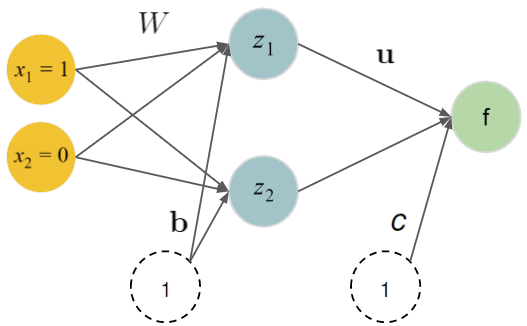
\includegraphics{figure/forwardprop1_new.png}}
      % \caption{A neural network with two neurons in the hidden layer. $W$ and $\biasb$ are the weights and biases of the hidden layer. $\wtu$ and $c$ are the weights and bias of the output layer. Based on the values for the weights (and biases), we will perform one forward and one backward pass.}
  \end{figure}
\begin{footnotesize}
  Note: We will only show rounded decimals. 
\end{footnotesize}
% \framebreak
\end{vbframe} 

\begin{vbframe}{ Forward pass}

\begin{itemize}
\item We will divide the FP into four steps:
\begin{itemize}
\item the inputs of $z_j$: $\bm{{z_{j,in}}}$
\item the activations of $z_j$: $\bm{{z_{j,out}}}$
\item the input of $f$: $\bm{{f_{in}}}$
\item and finally the activation of $f$: $\bm{{f_{out}}}$
\end{itemize}
\begin{figure}
\centering
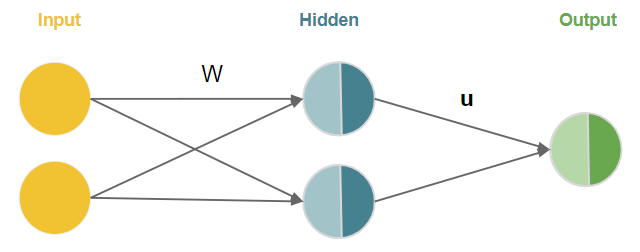
\includegraphics[width=8cm]{figure/xor_rep.png}
\end{figure}
\begin{figure}
\centering
\scalebox{0.5}{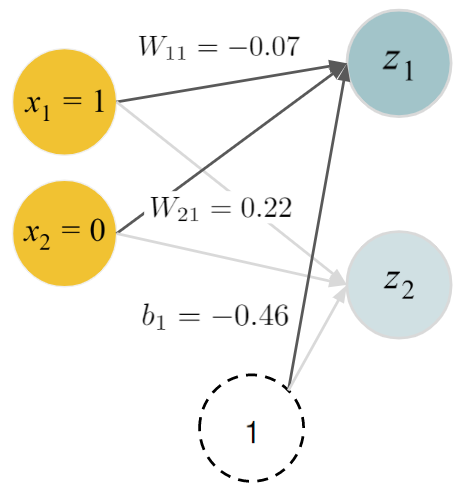
\includegraphics{figure/forwardprop2b_new.png}}
\end{figure}
\begin{footnotesize}
\begin{eqnarray*}
z_{1,in} &=& \Wmat_1^T \xv + b_1 =  1 \cdot (-0.07) + 0 \cdot 0.22 + 1 \cdot (-0.46) = -0.53 \\
z_{1,out} &=& \sigma\left(z_{1,in}\right) = \frac{1}{1+\exp(-(-0.53))} = \num[round-mode=places,round-precision=4]{0.3705169}
\end{eqnarray*}
\end{footnotesize}
\end{itemize}
\framebreak
%%%%%%%%%%%%%%%%%%%%%%%%%%%%%%%%%%%%%%%%%%%%%%%%%%%%%%%%%%%%%%%%%%

  \begin{figure}
    \centering
      \scalebox{0.5}{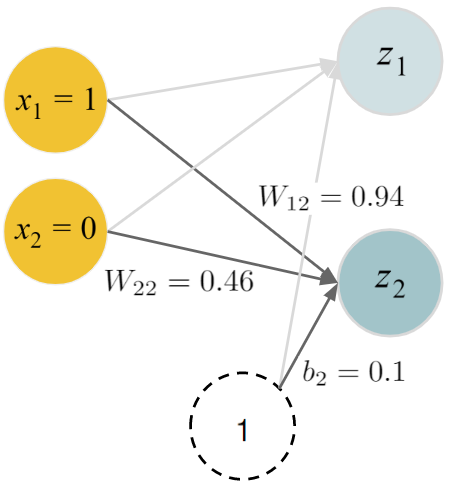
\includegraphics{figure/forwardprop3b_new.png}}
  \end{figure}
\vspace*{-0.5cm}
  \begin{footnotesize}
    \begin{eqnarray*}
    z_{2,in} &=& \Wmat_2^T \xv + b_2 = 1 \cdot 0.94 + 0 \cdot 0.46 + 1 \cdot 0.1 = 1.04 \\
    z_{2,out} &=& \sigma\left(z_{2,in}\right) = \frac{1}{1+\exp(-1.04)} = \num[round-mode=places,round-precision=4]{0.73885}
    \end{eqnarray*}
  \end{footnotesize}
\framebreak
%%%%%%%%%%%%%%%%%%%%%%%%%%%%%%%%%%%%%%%%%%%%%%%%%%%%%%%%%%%%%%%%%%

  \begin{figure}
    \centering
      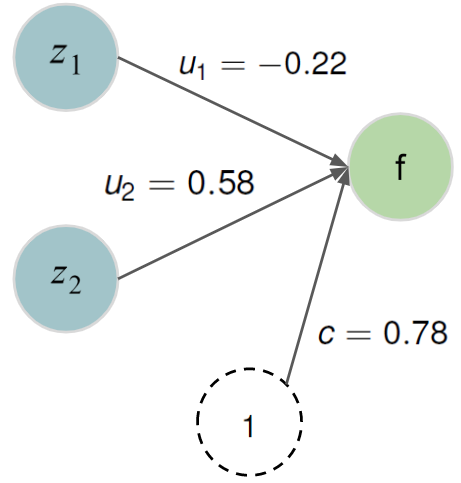
\includegraphics[width=5cm]{figure/forwardprop4b_new.png}
  \end{figure}

\vspace*{-0.5cm}

  \begin{footnotesize}
    \begin{eqnarray*}
    f_{in} &=& \bm{u}^T \bm{z} + c = \num[round-mode=places,round-precision=4]{0.3705169} \cdot (-0.22) + \num[round-mode=places,round-precision=4]{0.73885} \cdot 0.58 + 1 \cdot 0.78 = \num[round-mode=places,round-precision=4]{1.112242} \\
    f_{out} &=& \tau\left(f_{in}\right) = \frac{1}{1+\exp(\num[round-mode=places,round-precision=4]{-1.112242})} = \num[round-mode=places,round-precision=4]{0.7525469}
    \end{eqnarray*}
  \end{footnotesize}
\framebreak
%%%%%%%%%%%%%%%%%%%%%%%%%%%%%%%%%%%%%%%%%%%%%%%%%%%%%%%%%%%%%%%%%%

  \begin{itemize}
    \item The FP predicted $f_{out} = 0.7525$
    \item Now, we compare the prediction $f_{out} = 0.7525$ and the true label $y = 1$ using the L2-loss: 
      \begin{eqnarray*}
        \Lxy &=& \frac{1}{2}(y - \fxit)^2 = \frac{1}{2}\left(y - f_{out}\right)^{2} \\
                  &=& \frac{1}{2}\left(1 - \num[round-mode=places,round-precision=4]{0.7525469}\right)^2 = \num[round-mode=places,round-precision=4]{0.03061652}
      \end{eqnarray*}
    \item The calculation of the gradient is performed backwards (starting from the output layer), so that results can be reused. 
\end{itemize}
\end{vbframe}
%%%%%%%%%%%%%%%%%%%%%%%%%%%%%%%%%%%%%%%%%%%%%%%%%%%%%%%%%%%%%%%%%%

\begin{vbframe}{Backward pass}
% \begin{itemize}
   The main ingredients of the backward pass are: 
    \begin{itemize}
      \item to reuse the results of the forward pass \\ (here:  ${z_{j, in}, z_{j, out}, f_{in},f_{out}}$)
      \item reuse the \textcolor{violet}{intermediate results} from the chain rule 
      \item the derivative of the activations and some affine functions
    \end{itemize}
    % \item This is demonstrated by continuing the example above.
      % \end{itemize}
\framebreak
%%%%%%%%%%%%%%%%%%%%%%%%%%%%%%%%%%%%%%%%%%%%%%%%%%%%%%%%%%%%%%%%%%

  \begin{itemize}
    \item Let's start to update $u_1$. We recursively apply the chain rule: $$\frac{\partial \Lxy}{\partial u_1} = \frac{\partial \Lxy}{\partial f_{out}} \cdot \frac{\partial f_{out}}{\partial f_{in}} \cdot \frac{\partial f_{in}}{\partial u_1}$$
  \end{itemize}
  \begin{figure}
    \centering
      \scalebox{0.54}{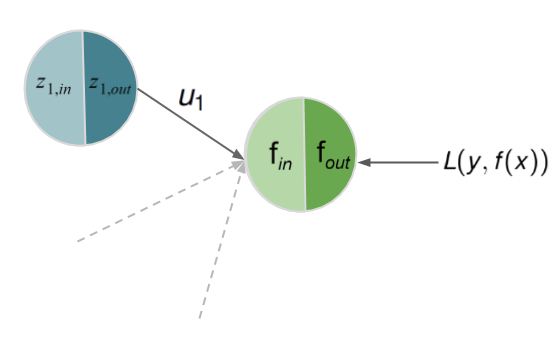
\includegraphics{figure/backprop1_new.png}}
      \caption{\footnotesize{Snippet from our NN, with backward path for $u_1$.}}
  \end{figure}
\framebreak
%%%%%%%%%%%%%%%%%%%%%%%%%%%%%%%%%%%%%%%%%%%%%%%%%%%%%%%%%%%%%%%%%%

  \begin{itemize}
    \item 1st step: The derivative of L2 is easy; we know ${f_{out}}$ from FP.
  \end{itemize}
    \begin{eqnarray*}
      \textcolor{violet}{\frac{\partial \Lxy}{\partial f_{out}}} &=& \frac{d}{\partial f_{out}} \frac{1}{2}(y - f_{out})^2 = -\underbrace{(y - {f_{out}})}_{\hat{=} \text{residual}} \\
       &=& -(1 - \num[round-mode=places,round-precision=4]{0.7525469}) = \num[round-mode=places,round-precision=4]{-0.2474531}
    \end{eqnarray*}
    \begin{figure}
      \centering
        \scalebox{0.6}{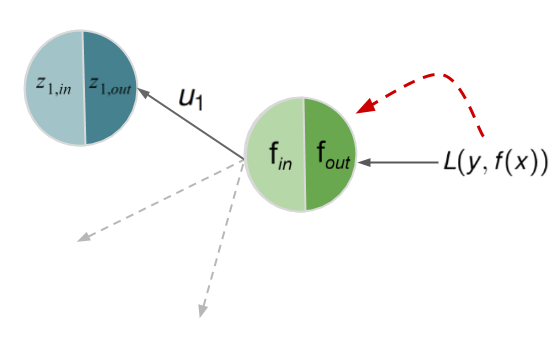
\includegraphics{figure/backprop1_b_new.png}}
        % \caption{The first term of our chain rule $\frac{\partial \Lxy}{\partial f_{out}}$}
    \end{figure}
\framebreak
%%%%%%%%%%%%%%%%%%%%%%%%%%%%%%%%%%%%%%%%%%%%%%%%%%%%%%%%%%%%%%%%%%

  \begin{itemize}
    \item 2nd step. $f_{out} = \sigma(f_{in})$, use rule for $\sigma'$, use ${f_{in}}$ from FP.
  \end{itemize}
    \begin{eqnarray*}
      \textcolor{violet}{\frac{\partial f_{out}}{\partial f_{in}}}  &=& \sigma({f_{in}})\cdot(1-\sigma({f_{in}})) \\
      &=& \num[round-mode=places,round-precision=4]{0.7525469} \cdot (1 - \num[round-mode=places,round-precision=4]{0.7525469}) = \num[round-mode=places,round-precision=4]{0.1862201}
    \end{eqnarray*}
      \vspace{-0.5cm}
    \begin{figure}
      \centering
        \scalebox{0.6}{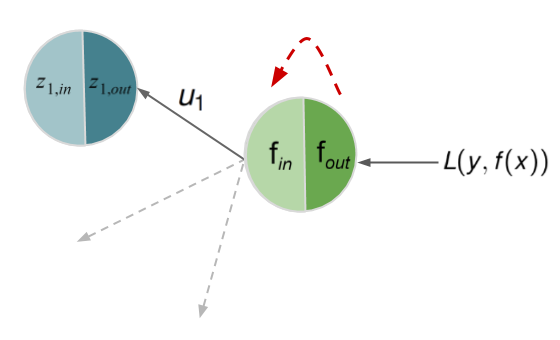
\includegraphics{figure/backprop1_c_new.png}}
        % \caption{The second term of our chain rule $\frac{\partial f_{out}}{\partial f_{in}}$}
    \end{figure}
\framebreak
%%%%%%%%%%%%%%%%%%%%%%%%%%%%%%%%%%%%%%%%%%%%%%%%%%%%%%%%%%%%%%%%%%

  \begin{itemize}
    \item 3rd step. Derivative of the linear input is easy; use ${z_{1, out}}$ from FP.
  \end{itemize}
    \begin{eqnarray*}
      \textcolor{violet}{\frac{\partial f_{in}}{\partial u_1}} = \frac{\partial (u_1 \cdot z_{1,out} + u_2 \cdot z_{2,out} + c \cdot 1)}{\partial u_1} = {z_{1, out}} = \num[round-mode=places,round-precision=4]{0.3705169}
    \end{eqnarray*}
    \begin{figure}
      \centering
        \scalebox{0.6}{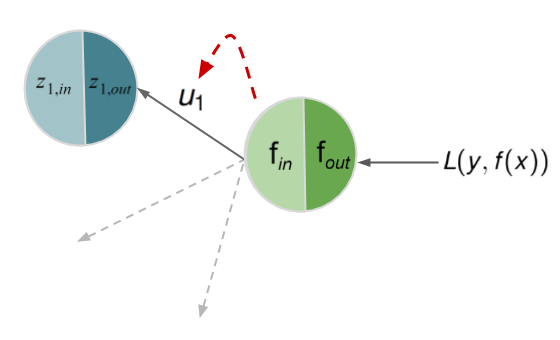
\includegraphics{figure/backprop1_d_new.png}}
        % \caption{The third term of our chain rule $\frac{\partial f_{in}}{\partial u_1}$}
    \end{figure}
\framebreak
%%%%%%%%%%%%%%%%%%%%%%%%%%%%%%%%%%%%%%%%%%%%%%%%%%%%%%%%%%%%%%%%%%

  \begin{itemize}
    \item Plug it together:
  \begin{eqnarray*}
    \textcolor{violet}{\frac{\partial \Lxy}{\partial u_1}} &=& \textcolor{violet}{\frac{\partial \Lxy}{\partial f_{out}}} \cdot \textcolor{violet}{\frac{\partial f_{out}}{\partial f_{in}}} \cdot \textcolor{violet}{\frac{\partial f_{in}}{\partial u_1}} \\
                                        &=& \num[round-mode=places,round-precision=4]{-0.2474531} \cdot \num[round-mode=places,round-precision=4]{0.1862201} \cdot \num[round-mode=places,round-precision=4]{0.3705169} = \num[round-mode=places,round-precision=4]{-0.01707369}
  \end{eqnarray*}
    \begin{figure}
      \centering
        \scalebox{0.4}{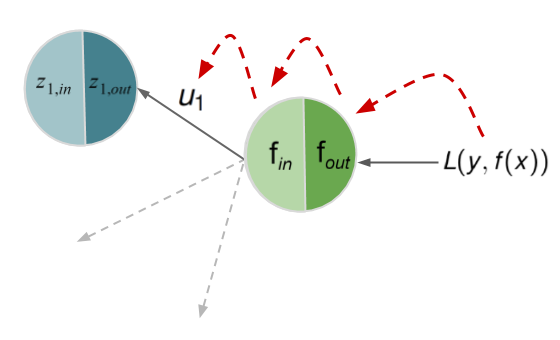
\includegraphics{figure/backprop1_e_new.png}}
        % \caption{All three terms of our chain rule $\frac{\partial \Lxy}{\partial u_1} = \frac{\partial \Lxy}{\partial f_{out}} \cdot \frac{\partial f_{out}}{\partial f_{in}} \cdot \frac{\partial f_{in}}{\partial u_1}$}
    \end{figure}
% \framebreak
%%%%%%%%%%%%%%%%%%%%%%%%%%%%%%%%%%%%%%%%%%%%%%%%%%%%%%%%%%%%%%%%%%

  % \begin{itemize}
\item  With LR $\alpha = 0.5$:
  % \end{itemize}
    \begin{eqnarray*}
      u_1^{[t+1]} &=& u_1^{[t]} - \alpha \cdot \textcolor{violet}{\frac{\partial \Lxy}{\partial u_1}} \\
                &=& -0.22 - 0.5 \cdot (\num[round-mode=places,round-precision=4]{-0.01707369}) = \num[round-mode=places,round-precision=4]{-0.2114632}
    \end{eqnarray*}
  \end{itemize}
\framebreak
%%%%%%%%%%%%%%%%%%%%%%%%%%%%%%%%%%%%%%%%%%%%%%%%%%%%%%%%%%%%%%%%%%

  \begin{itemize}
    \item Now for $W_{11}$: $$\frac{\partial \Lxy}{\partial W_{11}} = \textcolor{violet}{\frac{\partial \Lxy}{\partial f_{out}}} \cdot \textcolor{violet}{\frac{\partial f_{out}}{\partial f_{in}}} \cdot \frac{\partial f_{in}}{\partial z_{1,out}} \cdot \frac{\partial z_{1,out}}{\partial z_{1,in}} \cdot \frac{\partial z_{1,in}}{\partial W_{11}}$$
  \end{itemize}
  % \begin{figure}
    % \centering
      % \scalebox{0.70}{\includegraphics{figure/backprop2_new.png}}
      % \caption{Snippet from our neural network showing the backward path to compute the gradient with respect to weight $W_{11}$.}
  % \end{figure}
% \framebreak
%%%%%%%%%%%%%%%%%%%%%%%%%%%%%%%%%%%%%%%%%%%%%%%%%%%%%%%%%%%%%%%%%%

  \begin{itemize}
    \item We know $\textcolor{violet}{\frac{\partial \Lxy}{\partial f_{out}}}$ and $\textcolor{violet}{\frac{\partial f_{out}}{\partial f_{in}}}$ from BP for $u_1$.
  \begin{figure}
    \centering
      \scalebox{0.7}{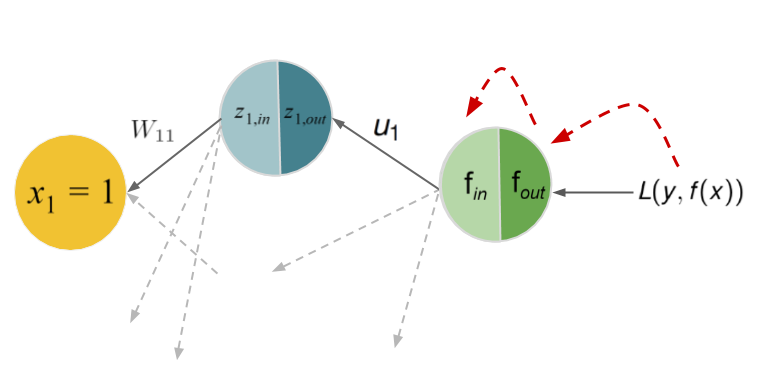
\includegraphics{figure/backprop2_bc_new.png}}
      % \caption{The first and second term of our chain rule $\frac{\partial \Lxy}{\partial f_{out}}$ and $\frac{\partial f_{out}}{\partial f_{in}}$}
  \end{figure}
\framebreak
%%%%%%%%%%%%%%%%%%%%%%%%%%%%%%%%%%%%%%%%%%%%%%%%%%%%%%%%%%%%%%%%%%

    \item $f_{in} = u_1 \cdot z_{1,out} + u_2 \cdot z_{2,out} + c \cdot 1$ is linear, easy and we know $u_1$ :
  \end{itemize}
  \begin{eqnarray*}
    \textcolor{violet}{\frac{\partial f_{in}}{\partial z_{1,out}}} = u_1 = -0.22
  \end{eqnarray*}
  \begin{figure}
    \centering
      \scalebox{0.7}{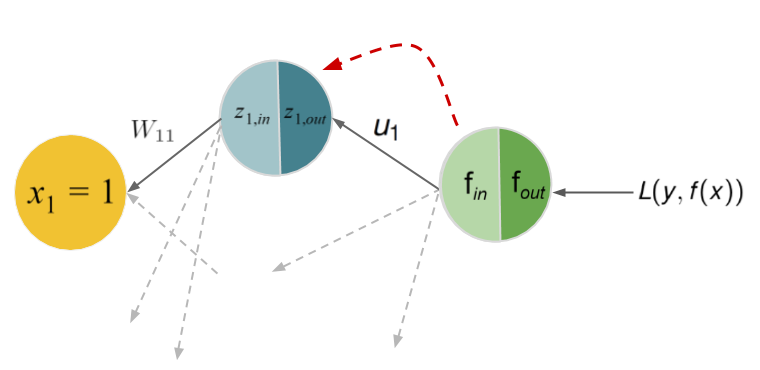
\includegraphics{figure/backprop2_d_new.png}}
      % \caption{The third term of our chain rule $\frac{\partial f_{in}}{\partial z_{1,out}}$}
  \end{figure}
\framebreak
%%%%%%%%%%%%%%%%%%%%%%%%%%%%%%%%%%%%%%%%%%%%%%%%%%%%%%%%%%%%%%%%%%

  \begin{itemize}
    \item Next. Use rule for $\sigma'$ and FP results:
  \end{itemize}
  \begin{eqnarray*}
    \textcolor{violet}{\frac{\partial z_{1,out}}{\partial z_{1,in}}}  &=& \sigma({z_{1,in}}) \cdot (1-\sigma({z_{1,in}})) \\&=&  \num[round-mode=places,round-precision=4]{0.3705169} \cdot (1 - \num[round-mode=places,round-precision=4]{0.3705169}) = \num[round-mode=places,round-precision=4]{0.2332341}
  \end{eqnarray*}
  \begin{figure}
    \centering
      \scalebox{0.7}{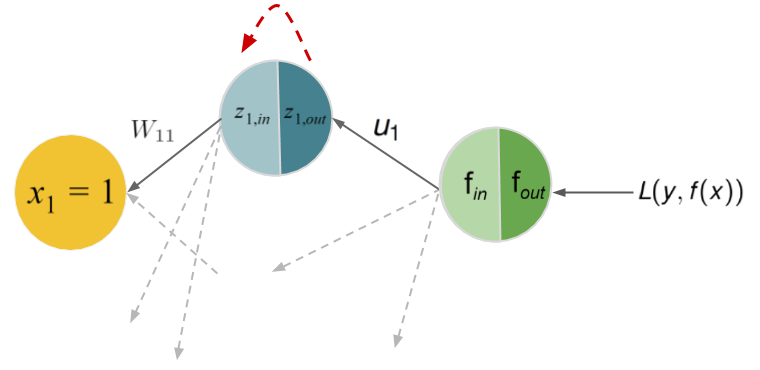
\includegraphics{figure/backprop2_e_new.png}}
      % \caption{The fourth term of our chain rule $\frac{\partial z_{1,out}}{\partial z_{1,in}}$}
  \end{figure}
\framebreak
%%%%%%%%%%%%%%%%%%%%%%%%%%%%%%%%%%%%%%%%%%%%%%%%%%%%%%%%%%%%%%%%%%

  \begin{itemize}
    \item $z_{1,in} = x_1 \cdot W_{11} + x_2 \cdot W_{21} + b_1 \cdot 1$ is linear
        and depends on inputs:
  \end{itemize}
  \begin{eqnarray*}
    \textcolor{violet}{\frac{\partial z_{1,in}}{\partial W_{11}}} = x_1 = 1
  \end{eqnarray*}
  \begin{figure}
    \centering
      \scalebox{0.65}{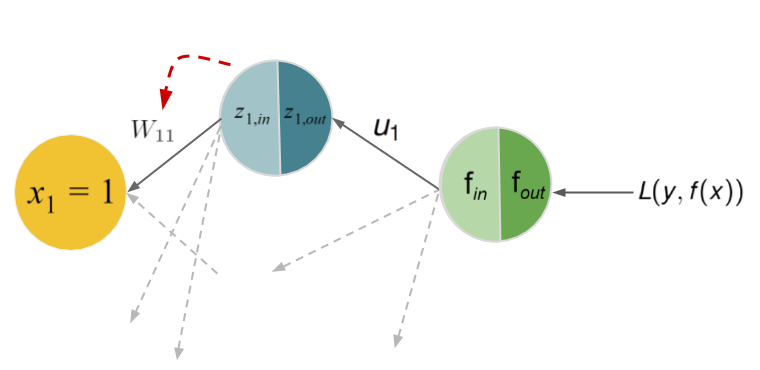
\includegraphics{figure/backprop2_f_new.png}}
      % \caption{The fifth term of our chain rule $\frac{\partial z_{1,in}}{\partial W_{11}}$}
  \end{figure}
\framebreak
%%%%%%%%%%%%%%%%%%%%%%%%%%%%%%%%%%%%%%%%%%%%%%%%%%%%%%%%%%%%%%%%%%

  \begin{itemize}
    \item Plugging together: 
      \begin{eqnarray*}
         \textcolor{violet}{\frac{\partial \Lxy}{\partial W_{11}}} &=& 
         \textcolor{violet}{\frac{\partial \Lxy}{\partial f_{out}}} \cdot  \textcolor{violet}{\frac{\partial f_{out}}{\partial f_{in}}} \cdot  \textcolor{violet}{\frac{\partial f_{in}}{\partial z_{1,out}}} \cdot  \textcolor{violet}{\frac{\partial z_{1,out}}{\partial z_{1,in}}} \cdot  \textcolor{violet}{\frac{\partial z_{1,in}}{\partial W_{11}}} 
        \\ &=& (\num[round-mode=places,round-precision=4]{-0.2474531}) \cdot \num[round-mode=places,round-precision=4]{0.1862201} \cdot (-0.22) \cdot \num[round-mode=places,round-precision=4]{0.2332341} \cdot 1 
        \\ &=& \num[round-mode=places,round-precision=4]{0.0023645}
      \end{eqnarray*}
  \begin{figure}
    \centering
      \scalebox{0.5}{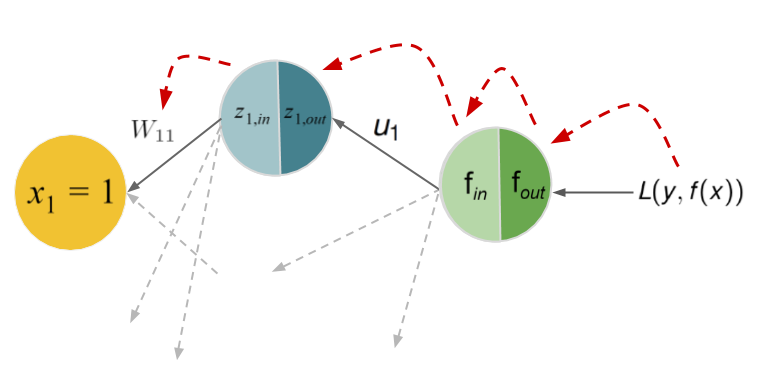
\includegraphics{figure/backprop2_g_new.png}}
      % \caption{All five terms of our chain rule}
  \end{figure}
% \framebreak
%%%%%%%%%%%%%%%%%%%%%%%%%%%%%%%%%%%%%%%%%%%%%%%%%%%%%%%%%%%%%%%%%%

    \item Full SGD update: 
    \begin{eqnarray*}
      W_{11}^{[t+1]}  &=& W_{11}^{[t]} - \alpha \cdot  \textcolor{violet}{\frac{\partial \Lxy}{\partial W_{11}}} \\
                  &=& -0.07 - 0.5 \cdot \num[round-mode=places,round-precision=4]{0.0023645} = \num[round-mode=places,round-precision=4]{-0.0711823}
    \end{eqnarray*}
  \end{itemize}
\end{vbframe}

\begin{vbframe}{Result}
  \begin{itemize}
    \item We can do this for all weights:
  \end{itemize}
  \begin{eqnarray*}
    \textbf{W} = \begin{pmatrix}
    \num[round-mode=places,round-precision=4]{-0.0711823} & \num[round-mode=places,round-precision=4]{0.9425785} \\
    0.22 & 0.46
    \end{pmatrix},
    \textbf{b} = \begin{pmatrix}
    \num[round-mode=places,round-precision=4]{-0.4611822} \\
    \num[round-mode=places,round-precision=4]{0.1025782}
    \end{pmatrix},
  \end{eqnarray*}
  \begin{eqnarray*}
    \textbf{u} = \begin{pmatrix}
    \num[round-mode=places,round-precision=4]{-0.2114632} \\
    \num[round-mode=places,round-precision=4]{0.5970234}
    \end{pmatrix}
    \text{and} \ c = \num[round-mode=places,round-precision=4]{0.8030404}\text{.}
  \end{eqnarray*}
% \framebreak  
%%%%%%%%%%%%%%%%%%%%%%%%%%%%%%%%%%%%%%%%%%%%%%%%%%%%%%%%%%%%%%%%%%

  \begin{itemize}
    \item Yields $f(\xv ~|~\thetav^{[t+1]}) = \num[round-mode=places,round-precision=4]{0.7614865}$ and loss 
        $\frac{1}{2}(1 - \num[round-mode=places,round-precision=4]{0.7614865})^2 = \num[round-mode=places,round-precision=4]{0.02844434}.$
        % $\Lxy = \frac{1}{2}(1 - \num[round-mode=places,round-precision=4]{0.7614865})^2 = \num[round-mode=places,round-precision=4]{0.02844434}.$$
    \item Before, we had $f(\xv ~|~\thetav^{[t]}) = \num[round-mode=places,round-precision=4]{0.7525469}$ and higher loss $\num[round-mode=places,round-precision=4]{0.03061652}$.

  \end{itemize}
\lz
 Now rinse and repeat. This was one training iter, we do thousands.
\end{vbframe}
%%%%%%%%%%%%%%%%%%%%%%%%%%%%%%%%%%%%%%%%%%%%%%%%%%%%%%%%%%%%%%%%%%

% \begin{frame} { Summary}
%   \begin{itemize}
%     \item Our goal was to minimize the true/expected risk $$\riskt = \E_{(\xv, y)\sim \Pxy} \left[\Lxyt\right]$$
%     with respect to the true underlying distribution $\Pxy$.
%     \item Because we do not know $\Pxy$, we decided to minimize the empirical risk $$\risket = \frac{1}{n} \sumin \Lxyit$$ w.r.t. the training set and hope for the best.
%     \item However, even this is not possible because there is no way to analytically find a global minimum for deep neural networks.
%     \item Therefore, we decided to use gradient descent to iteratively find a local minimum of the (typically) non-convex loss function.
%   \end{itemize}
% \end{frame}
%%%%%%%%%%%%%%%%%%%%%%%%%%%%%%%%%%%%%%%%%%%%%%%%%%%%%%%%%%%%%%%%%%

% \begin{frame} { Summary}
  % \begin{itemize}
      % \item To perform gradient descent, we want to compute the gradient of the loss function $\risket$ with respect to \textbf{all} the weights and biases in the network.
      % \item Therefore, the number of components in the gradient is the total number of weights and biases in the network.
      % \item To compute each component of the gradient, we apply the chain rule to the relevant portion of the computational graph.
      % \item In software, a vectorized version of the chain rule is used to compute the derivatives w.r.t. multiple weights simultaneously.
      % \item Loosely speaking, each term in the gradient represents the extent to which the corresponding weight is responsible for the loss. In other words, it is a way to assign "blame" to each weight.
  % \end{itemize}
% \end{frame}
%%%%%%%%%%%%%%%%%%%%%%%%%%%%%%%%%%%%%%%%%%%%%%%%%%%%%%%%%%%%%%%%%%

% \begin{vbframe} { Summary}

  % \begin{itemize}
    % \item Gradient descent can be implemented efficiently: 
    % \begin{itemize}
      % \item We can store and reuse results of the forward pass
      % \item We reuse intermediate results from the chain rule during the BP.  
      % \item We know how derivates of activation functions and affine functions look like
    % \end{itemize}
    % For example, to compute the derivative of the sigmoid activation at $z_{1,out}$, we \enquote{stored} the derivative of the sigmoid function $\frac{\partial z_{1,out}}{\partial z_{1,in}} = \sigma(z_{1,in})(1-\sigma(z_{1,in}))$ and plugged in $\sigma(z_{1,in}) = \num[round-mode=places,round-precision=4]{0.3705169}$, which was known from the forward pass.
% \end{itemize}
% \framebreak  
%%%%%%%%%%%%%%%%%%%%%%%%%%%%%%%%%%%%%%%%%%%%%%%%%%%%%%%%%%%%%%%%%%

  % \begin{itemize}
  % \item In our example, we updated w.r.t. a single training example but typically, we feed subsets of the training set (minibatch GD).
    % \item The term \enquote{backpropagation} refers to the fact that the computation of the gradient using the chain rule is performed backwards (that is, starting at the output layer and finishing at the first hidden layer). 
      % A \textbf{forward} computation using the chain rule also results in the same gradient but can be computationally expensive (see http://colah.github.io/posts/2015-08-Backprop/).
 % \end{itemize}
% \end{frame} 
%%%%%%%%%%%%%%%%%%%%%%%%%%%%%%%%%%%%%%%%%%%%%%%%%%%%%%%%%%%%%%%%%%

% \begin{frame} { Summary}
%   \begin{itemize}
%     \item After computing the gradient (using backpropagation), we subtract the gradient (scaled by the learning-rate $\alpha$) from the current set of weights (and biases) which results in a new set of weights (and biases).
%     \item The empirical loss for this new set of weights is now lower ("walking down the hill").
%     \item Next, we once again compute the forward pass for this new set of weights and store the activations.
%     \item Then, we compute the gradient of the empirical loss using backpropagation and take another step down the hill.
%     \item Rinse and repeat (until the loss stops decreasing substantially). 
%       However, training until convergence often results in overfitting (use early stopping).
%   \end{itemize}
% \end{frame}
%%%%%%%%%%%%%%%%%%%%%%%%%%%%%%%%%%%%%%%%%%%%%%%%%%%%%%%%%%%%%%%%%%


\section{Basic Backpropagation 2}
%%%%%%%%%%%%%%%%%%%%%%%%%%%%%%%%%%%%%%%%%%%%%%%%%%%%%%%%%%%%%%%%%%


\begin{frame} {Backward Computation and Caching}
    In the XOR example, we computed:
    $$\frac{\partial \Lxy}{\partial W_{11}} = 
        \frac{\partial \Lxy}{\partial f_{out}} \cdot  \textcolor{black}{\frac{\partial f_{out}}{\partial f_{in}}} \cdot  \textcolor{black}{\frac{\partial f_{in}}{\partial z_{1,out}}} \cdot  \textcolor{black}{\frac{\partial z_{1,out}}{\partial z_{1,in}}} \cdot  \textcolor{black}{\frac{\partial z_{1,in}}{\partial W_{11}}} $$
  \begin{figure}
    \centering
      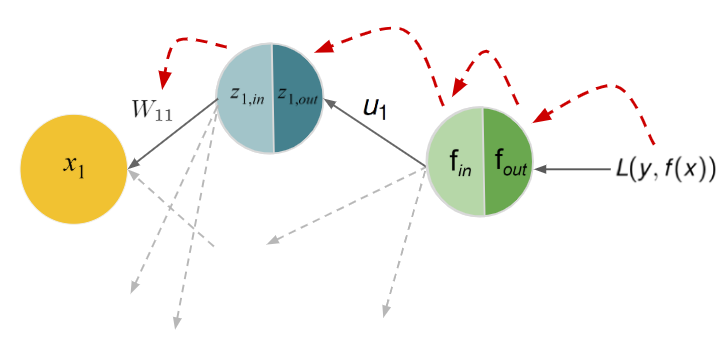
\includegraphics[width=9cm]{figure/backprop_gg1_new.png}
      % \caption{All five terms of our chain rule}
  \end{figure}
\end{frame}
%%%%%%%%%%%%%%%%%%%%%%%%%%%%%%%%%%%%%%%%%%%%%%%%%%%%%%%%%%%%%%%%%%

\begin{frame} {Backward Computation and Caching}
Next, let us compute:
      $$\frac{\partial \Lxy}{\partial W_{21}} = 
\frac{\partial \Lxy}{\partial f_{out}} \cdot  \textcolor{black}{\frac{\partial f_{out}}{\partial f_{in}}} \cdot  \textcolor{black}{\frac{\partial f_{in}}{\partial z_{1,out}}} \cdot  \textcolor{black}{\frac{\partial z_{1,out}}{\partial z_{1,in}}} \cdot  \textcolor{black}{\frac{\partial z_{1,in}}{\partial W_{21}}}$$
        \begin{figure}
    \centering
      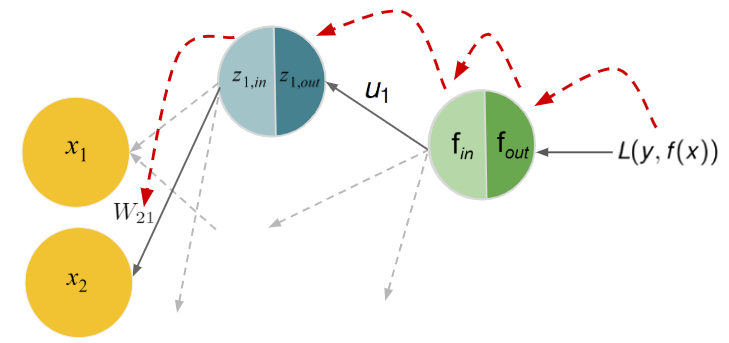
\includegraphics[width=9cm]{figure/backprop_gg_new.png}
      % \caption{All five terms of our chain rule}
  \end{figure}
\end{frame}
%%%%%%%%%%%%%%%%%%%%%%%%%%%%%%%%%%%%%%%%%%%%%%%%%%%%%%%%%%%%%%%%%%

\begin{frame} {Backward Computation and Caching}
\begin{itemize}
\item Examining the two expressions:
$$\frac{\partial \Lxy}{\partial W_{11}} = 
\textcolor{violet}{\frac{\partial \Lxy}{\partial f_{out}}} \cdot  \textcolor{violet}{\frac{\partial f_{out}}{\partial f_{in}}} \cdot  \textcolor{violet}{\frac{\partial f_{in}}{\partial z_{1,out}}} \cdot  \textcolor{violet}{\frac{\partial z_{1,out}}{\partial z_{1,in}}} \cdot  \textcolor{black}{\frac{\partial z_{1,in}}{\partial W_{11}}}$$

$$\frac{\partial \Lxy}{\partial W_{21}} =     
\textcolor{violet}{\frac{\partial \Lxy}{\partial f_{out}}} \cdot  \textcolor{violet}{\frac{\partial f_{out}}{\partial f_{in}}} \cdot  \textcolor{violet}{\frac{\partial f_{in}}{\partial z_{1,out}}} \cdot  \textcolor{violet}{\frac{\partial z_{1,out}}{\partial z_{1,in}}} \cdot  \textcolor{black}{\frac{\partial z_{1,in}}{\partial W_{21}}}$$

\item Significant overlap / redundancy in the two expressions.
\item \textbf{Again}: Let's call this subexpression $\delta_1$ and cache it.
    % Simply cache these subexpressions instead of recomputing them each time.
% \end{itemize}
% \end{frame}
%%%%%%%%%%%%%%%%%%%%%%%%%%%%%%%%%%%%%%%%%%%%%%%%%%%%%%%%%%%%%%%%%%

% \begin{frame} {Backward Computation and Caching}
% \begin{itemize}
{\small $$\textcolor{violet}{\delta_1}  = \textcolor{violet}{\frac{\partial \Lxy}{\partial z_{1,in}}} = 
\textcolor{violet}{\frac{\partial \Lxy}{\partial f_{out}}} \cdot  \textcolor{violet}{\frac{\partial f_{out}}{\partial f_{in}}} \cdot  \textcolor{violet}{\frac{\partial f_{in}}{\partial z_{1,out}}} \cdot  \textcolor{violet}{\frac{\partial z_{1,out}}{\partial z_{1,in}}}$$} 
% \item  two expressions of the previous slide now become,
{\small $$\frac{\partial \Lxy}{\partial W_{11}} = \textcolor{violet}{\delta_1} \cdot \frac{\partial z_{1,in}}{\partial W_{11}} \mbox{ \hspace{0.5cm} \small{and} \hspace{0.5cm}} \frac{\partial \Lxy}{\partial W_{21}} = \textcolor{violet}{\delta_1} \cdot \frac{\partial z_{1,in}}{\partial W_{21}} $$}
\item $\delta_1$ can also be seen as an \textbf{error signal} that represents how much the loss $L$ changes when the input $z_{1,in}$ changes.

% where $\delta_1$ is simply "plugged in".
% \item As you can imagine, caching subexpressions in this way and plugging in where needed can result in \textbf{massive} gains in efficiency for deep and "wide" neural networks. 
% \item In fact, this simple algorithm, which was first applied to neural networks way back in 1985, is \textbf{still} the biggest breakthrough in deep learning.
\end{itemize}
\end{frame}
%%%%%%%%%%%%%%%%%%%%%%%%%%%%%%%%%%%%%%%%%%%%%%%%%%%%%%%%%%%%%%%%%%

% \begin{frame} {Backward Computation and Caching}
  % \begin{itemize}
  %   \item On the other hand, if we had done a \textbf{forward} caching of the derivatives
  %   {\small $$\frac{\partial \Lxy}{\partial W_{11}} = \Bigg(\Bigg(\Bigg( \frac{\partial z_{1,in}}{\partial W_{11}} \frac{\partial z_{1,out}}{\partial z_{1,in}} \Bigg)  \frac{\partial f_{in}}{\partial z_{1,out}} \Bigg) \frac{\partial f_{out}}{\partial f_{in}} \Bigg) \frac{\partial \Lxy}{\partial f_{out}}$$}
  %     {\small $$\frac{\partial \Lxy}{\partial W_{21}} = 
  %       \Bigg(\Bigg(\Bigg( \frac{\partial z_{1,in}}{\partial W_{21}} \frac{\partial z_{1,out}}{\partial z_{1,in}} \Bigg)  \frac{\partial f_{in}}{\partial z_{1,out}} \Bigg) \frac{\partial f_{out}}{\partial f_{in}} \Bigg) \frac{\partial \Lxy}{\partial f_{out}}$$}
  %     there would be no common subexpressions to plug in. We would have to compute the \text{entire} expression for each and every weight!
  %   \item This would make the computations too inefficient to make gradient descent tractable for large neural networks.
  % \end{itemize}
% \end{frame}
%%%%%%%%%%%%%%%%%%%%%%%%%%%%%%%%%%%%%%%%%%%%%%%%%%%%%%%%%%%%%%%%%%



\begin{frame} {Backprop: Recursion}
  \begin{itemize}
    \item \small{Let us now derive a general formulation of backprop.}
    \item \small{The neurons in layers $i-1$, $i$ and $i+1$ are indexed by $j$, $k$ and $m$, respectively.
    \item The output layer will be referred to as layer O.}
   \begin{figure}
    \centering
      \scalebox{0.8}{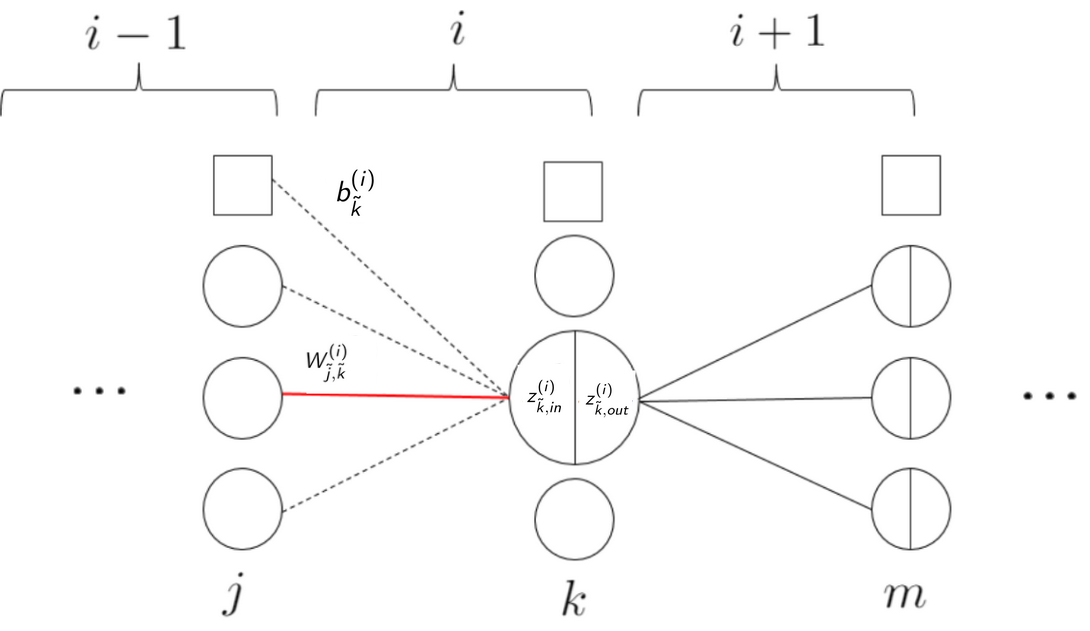
\includegraphics{figure/backnet.png}}
      %\tiny{\\Credit: Erik Hallstr\"{o}m}
      \caption{(Hallstr\"{o}m, 2016)}
    \end{figure}
  \end{itemize}
\end{frame}
%%%%%%%%%%%%%%%%%%%%%%%%%%%%%%%%%%%%%%%%%%%%%%%%%%%%%%%%%%%%%%%%%%

\begin{vbframe} {Backprop: Recursion}

  \vspace*{-0.3cm}

 \begin{figure}
  \centering
    \scalebox{0.6}{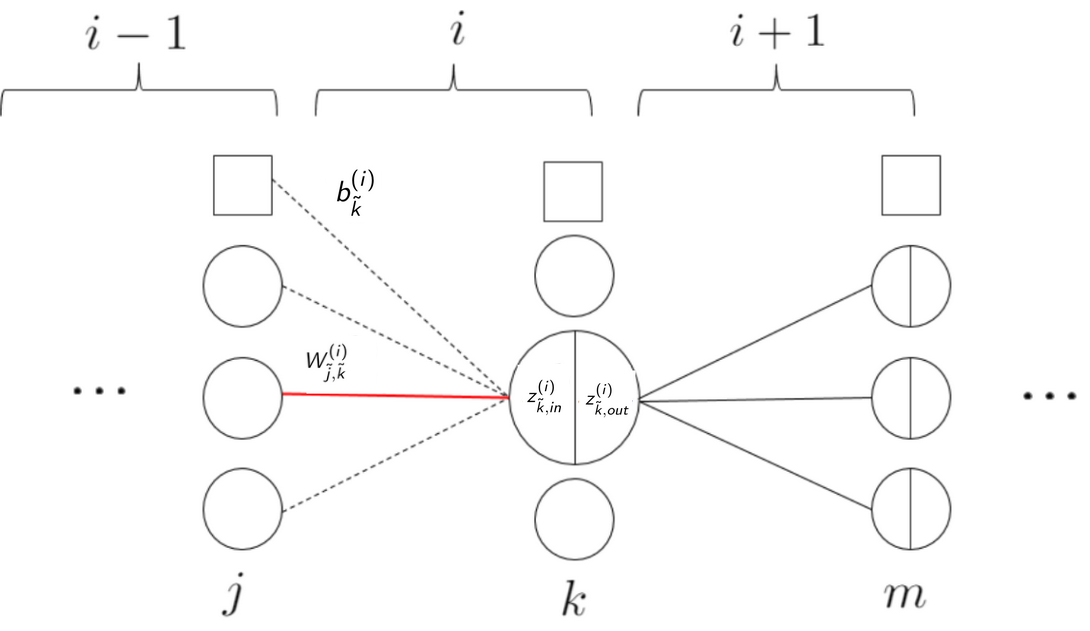
\includegraphics{figure/backnet.png}}
  \end{figure}
  \vspace*{-0.5cm}
  \begin{small}
  \begin{itemize}
    \item Let $\delta_{\tilde{k}}^{(i)}$ (also: error signal) for a neuron $\tilde{k}$ in layer $i$ represent how much the loss $L$ changes when the input $z_{\tilde{k},in}^{(i)}$   changes:
    {\small
      $$\delta_{\tilde{k}}^{(i)} = \frac{\partial L}{\partial z_{\tilde{k},in}^{(i)}} =  \frac{\partial L}{\partial z_{\tilde{k},out}^{(i)}} \frac{\partial z_{\tilde{k},out}^{(i)}}{\partial z_{\tilde{k},in}^{(i)}}   =  \sum_m \Bigg( \frac{\partial L}{\partial z_{m,in}^{(i+1)}} \frac{\partial z_{m,in}^{(i+1)}}{\partial z_{\tilde{k},out}^{(i)}} \Bigg) \frac{\partial z_{\tilde{k},out}^{(i)}}{\partial z_{\tilde{k},in}^{(i)}} $$}

    \item Note: The sum in the expression above is over all the neurons in layer $i+1$. This is simply an application of the (multivariate) chain rule.
  \end{itemize}
  \end{small}
\end{vbframe}
%%%%%%%%%%%%%%%%%%%%%%%%%%%%%%%%%%%%%%%%%%%%%%%%%%%%%%%%%%%%%%%%%%

\begin{frame} {Backprop: Recursion}
 Using 
 \vspace*{-5mm}
        {\footnotesize \begin{eqnarray*}
          \textcolor{blue}{z_{\tilde{k},out}^{(i)}} &=& \textcolor{blue}{\sigma(z_{\tilde{k},in}^{(i)})} \\
          \textcolor{violet}{z_{m,in}^{(i+1)}} &=& \textcolor{violet}{\sum_k W_{k,m}^{(i+1)}z_{k,out}^{(i)} + b_m^{(i+1)}}
        \end{eqnarray*}}
we get: 
      \vspace{-0.2cm}
      {\footnotesize \begin{eqnarray*}
      \delta_{\tilde{k}}^{(i)} &=& \sum_m \Bigg( \frac{\partial L}{\partial z_{m,in}^{(i+1)}} \frac{\partial \textcolor{violet}{z_{m,in}^{(i+1)}}}{\partial z_{\tilde{k},out}^{(i)}} \Bigg) \frac{\partial \textcolor{blue}{z_{\tilde{k},out}^{(i)}}}{\partial z_{\tilde{k},in}^{(i)}}  \\
       &=& \sum_m \Bigg( \frac{\partial L}{\partial z_{m,in}^{(i+1)}} \frac{\partial \left(\textcolor{violet}{\sum_k W_{k,m}^{(i+1)}z_{k,out}^{(i)} + b_m^{(i+1)}}\right)}{\partial z_{\tilde{k},out}^{(i)}} \Bigg) \frac{\partial \textcolor{blue}{\sigma(z_{\tilde{k},in}^{(i)})}}{\partial z_{\tilde{k},in}^{(i)}}  \\
      &=& \sum_m \Bigg( \frac{\partial L}{\partial z_{m,in}^{(i+1)}} \textcolor{violet}{W_{\tilde{k},m}^{(i+1)}} \Bigg) \textcolor{blue}{\sigma'(z_{\tilde{k},in}^{(i)})} = \sum_m \Bigg(  \delta_{\tilde{k}}^{(i+1)} \textcolor{violet}{W_{\tilde{k},m}^{(i+1)}} \Bigg) \textcolor{blue}{\sigma'(z_{\tilde{k},in}^{(i)})} 
      \end{eqnarray*}}\\
      Therefore, we now have a \textbf{recursive definition} for the error signal of a neuron in layer $i$ in terms of the error signals of the neurons in layer $i+1$ and, by extension, layers \{i+2, i+3 \ldots , O\}!
\end{frame}
%%%%%%%%%%%%%%%%%%%%%%%%%%%%%%%%%%%%%%%%%%%%%%%%%%%%%%%%%%%%%%%%%%

\begin{frame} {Backprop: Recursion}
  \begin{itemize}
    \item Given the error signal $\delta_{\tilde{k}}^{(i)}$ of neuron $\tilde{k}$ in layer $i$, the derivative of loss $L$ w.r.t. to the weight $W_{\tilde{j},\tilde{k}}$ is simply:
        $$
           \frac{\partial L}{\partial W_{\tilde{j},\tilde{k}}^{(i)}} = \frac{\partial L}{\partial z_{\tilde{k},in}^{(i)}} \frac{\partial z_{\tilde{k},in}^{(i)}}{\partial W_{\tilde{j},\tilde{k}}^{(i)}} 
           = \delta_{\tilde{k}}^{(i)} z_{\tilde{j},out}^{(i-1)} $$
        because $z_{\tilde{k},in}^{(i)} = \sum_j W_{j,\tilde{k}}^{(i)}z_{j,out}^{(i-1)}  + b_{\tilde{k}}^{(i)}$
    \item Similarly, the derivative of loss $L$ w.r.t. bias $b_{\tilde{k}}^{(i)}$ is:
      $$ \frac{\partial L}{\partial b_{\tilde{k}}^{(i)}} = \frac{\partial L}{\partial z_{\tilde{k},in}^{(i)}} \frac{\partial z_{\tilde{k},in}^{(i)}}{\partial b_{\tilde{k}}^{(i)}} = \delta_{\tilde{k}}^{(i)}$$
  \end{itemize}
\end{frame}
%%%%%%%%%%%%%%%%%%%%%%%%%%%%%%%%%%%%%%%%%%%%%%%%%%%%%%%%%%%%%%%%%%

\begin{frame} {Backprop: Recursion}
\begin{itemize}
\item It is not hard to show that the error signal $\bm{\delta}^{i}$ for an entire layer $i$ is ($\odot$ = element-wise product):
\begin{itemize}
\item $\bm{\delta}^{(O)} = \nabla_{f_{out}}L \odot \tau'(f_{in})$
\item $\bm{\delta}^{(i)} = W^{(i+1)}\bm{\delta}^{(i+1)} \odot \sigma'(z_{in}^{(i)})$
\end{itemize}
% \item As we have seen earlier, the error signal for a given layer $i$ depends recursively on the error signals of \textbf{later} layers \{i+1, i+2, \ldots , O\}.
\item Therefore, backpropagation works by computing and storing the error signals \textbf{backwards}. That is, starting at the output layer and ending at the first hidden layer. This way, the error signals of later layers \textbf{propagate backwards} to the earlier layers.
\item The derivative of the loss $L$ w.r.t. a given weight is computed efficiently by plugging in the cached error signals, thereby avoiding expensive and redundant computations. 
\end{itemize}
\end{frame}
%%%%%%%%%%%%%%%%%%%%%%%%%%%%%%%%%%%%%%%%%%%%%%%%%%%%%%%%%%%%%%%%%%

%%%%%%%%%%%%%%%%%%%%%%%%%%%%%%%%%%%%%%%%%%%%%%%%%%%%%%%%%%%%%%%%%%
%%%%%%%%%%%%%%%%%%%%%%%%%%%%%%%%%%%%%%%%%%%%%%%%%%%%%%%%%%%%%%%%%%
%%%%%%%%%%%%%%%%%%          REFERENCES          %%%%%%%%%%%%%%%%%%
%%%%%%%%%%%%%%%%%%%%%%%%%%%%%%%%%%%%%%%%%%%%%%%%%%%%%%%%%%%%%%%%%%
\begin{vbframe}
\frametitle{References}
\footnotesize{
\begin{thebibliography}{99}
%%%%%%%%%%%%%%%%%%%%%%%%%%%%%%%%%%
\bibitem[(Hallström, 2016)]{bp21} 
Hallström, E. (2016, December 4). \textit{Backpropagation from the beginning}. Medium. \url{https://medium.com/@erikhallstrm/backpropagation-from-the-beginning-77356edf427d} 
%%%%%%%%%%%%%%%%%%%%%%%%%%%%%%%%%%
\end{thebibliography}
}
\end{vbframe}



\section{Network Initializations}

%%%%%%%%%%%%%%%%%%%%%%%%%%%%%%%%%%%%%%%%%%%%%%%%%%%%%%%%%%%%%%%%%%
\begin{vbframe} {Practical Initialization}
  \begin{itemize}
    \item The weights (and biases) of a neural network must be assigned some initial values before training can begin.
    \item The choice of the initial weights (and biases) is crucial as it determines whether an optimization algorithm converges, how fast and whether to a point with high or low risk. 
    \item Initialization strategies to achieve "nice" properties are difficult to find, because there is no good understanding which properties are preserved under which circumstances. 
    \item In the following we seperate between the initialization of weights and biases. 
  \end{itemize}
  \end{vbframe}
  
%%%%%%%%%%%%%%%%%%%%%%%%%%%%%%%%%%%%%%%%%%%%%%5
\begin{vbframe}{Weight Initialization}
  \begin{itemize}
    \item It is important to initialize the weights randomly in order to "break symmetry". If two neurons (with the same activation function in a fully connected network) are connected to the same inputs and have the same initial weights, then both neurons will have the same gradient update in a given iteration and they will end up learning the same features.
    \item Furthermore, the initial weights should not be too large, because this might result in an explosion of weights or high sensitivity to changes in the input.
    \item Weights are typically drawn from a uniform distribution or a Gaussian centered at 0 with a small variance.
    \item Centering the initial weights around 0 can be seen as a form of regularization and it imposses that it is more likely that units do not interact with each other than they do interact.
    \framebreak
    \item Two common initialization strategies for weights are the 'Glorot initialization' and 'He initialization' which tune the variance of these distributions based on the topology of the network. %However, these strategies depend on the layer size and the initial weights can get extremely small with larger layer sizes.
    \item \textbf{Glorot initialization} suggests to sample each weight of a fully connected layer with $m$ inputs and $n$ outputs from a uniform distribution
    \begin{equation*}
      w_{j,k} \sim U\left(-\sqrt{\frac{6}{m+n}},\sqrt{\frac{6}{m+n}}\right)
    \end{equation*}
   The strategy is derived from the assumption that the network consists only of a chain of matrix multiplications with no nonlinearities. 
    \item \textbf{He initialization} is especially useful for neural networks with ReLU activations. Each weight of a fully connected layer with $m$ inputs is sampled from a Gaussian distribution 
    \begin{equation*}
      w_{j, k} \sim N\left(0, \frac{2}{m}\right)
    \end{equation*}
    The underlying derivation can be found in He et. al. (2015).
    \item Since the initialization strategies of Glorot and He depend on the layer sizes, the initial weights for large layer sizes can become extremely small.
    \item Another strategy is to treat the weights as hyperparameters that can be optimized by hyperparameter search algorithms. This can be computationally costly. 
    %\item Another strategy is to manually search for optimal weights by looking at the range or standard deviations of activations and gradients on a single minibatch. If the weights are too small, the range of the activations shrinks and the weights should be manually increased.
  \end{itemize}
\end{vbframe}

%%%%%%%%%%%%%%%%%%%%%%%%%%%%%%%%%%%%%%%%%%%%%%%%%%%%%%%%%%%%%%%%%%
\begin{vbframe}{Weight initialization: Example}
\begin{itemize}
\item We use a spiral planar data set to compare the following strategies: \\
Zero initialization, random initialization (samples from $N\left(0, 1\cdot 10^{-4}\right)$) and He initialization. 
\item For each strategy, a neural network with one hidden layer with 100 units, ReLU activation and Gradient Descent as optimizer was used. 
\end{itemize}
  \begin{figure}
  \vspace{-0.5cm}
    \centering
      \scalebox{0.4}{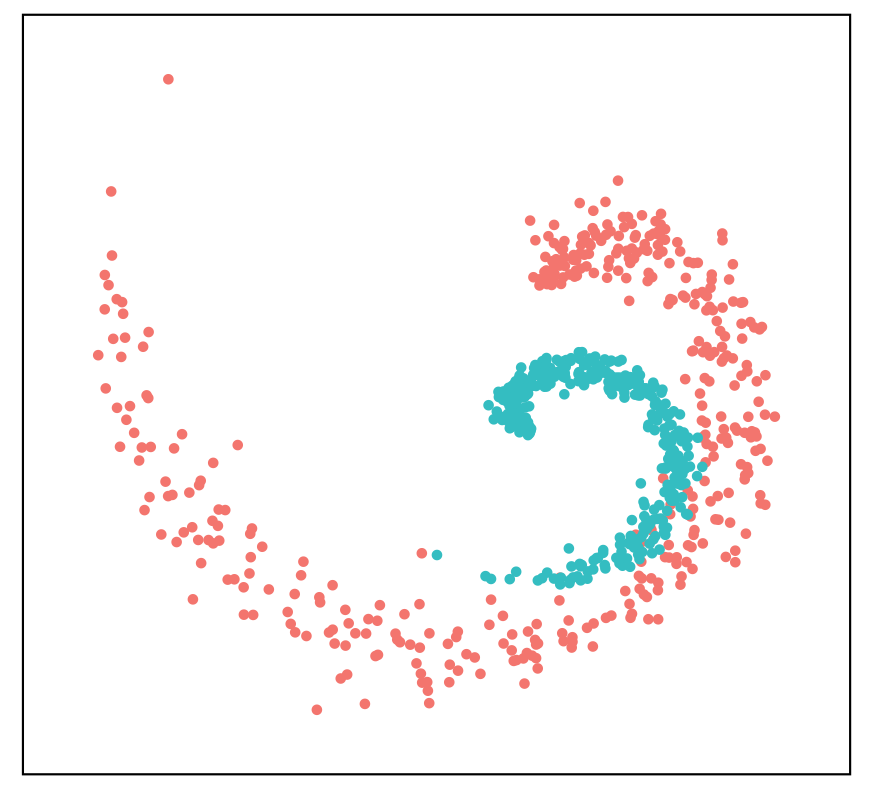
\includegraphics{figure/spiral_planar_data/data.png}}
      \caption{Simulated spiral planar data set with two classes (Ghatak, 2019).}
  \end{figure}
  \framebreak
  \begin{figure}
    \centering
      \scalebox{1}{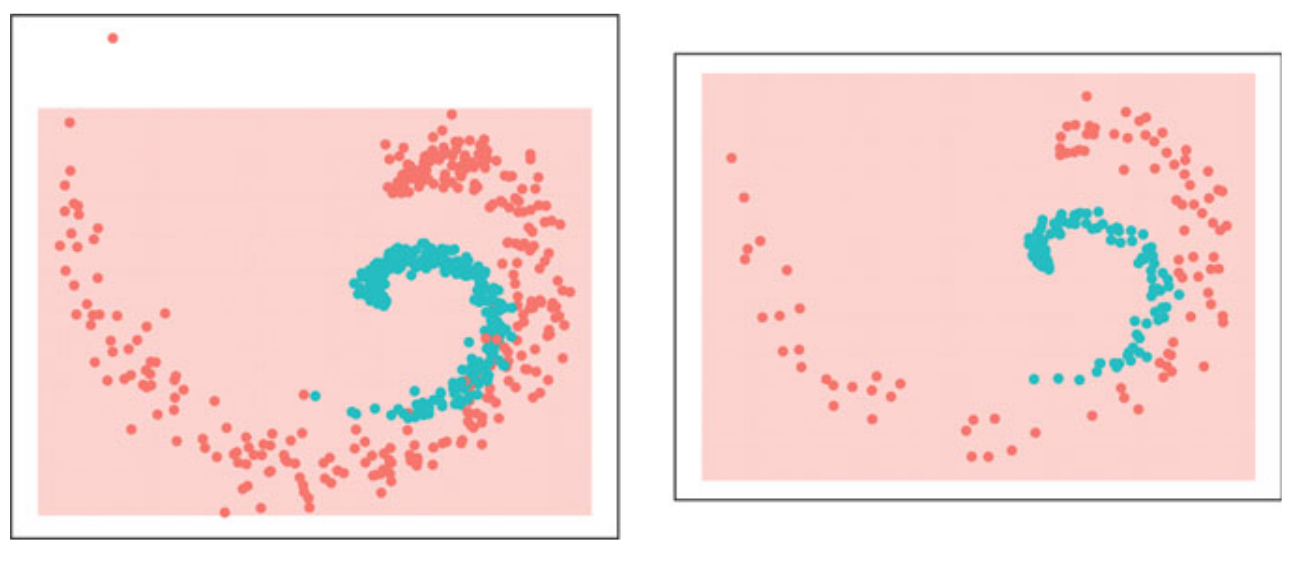
\includegraphics{figure/spiral_planar_data/zero.png}}
      \caption{Decision boundary with zero initialization on the training data set (left) and the testing data set (right). The zero initialization does not break symmetry and the complexity of the network reduces to that of a single
neuron (Ghatak, 2019).}
  \end{figure}
    \framebreak
  \begin{figure}
    \centering
      \scalebox{1}{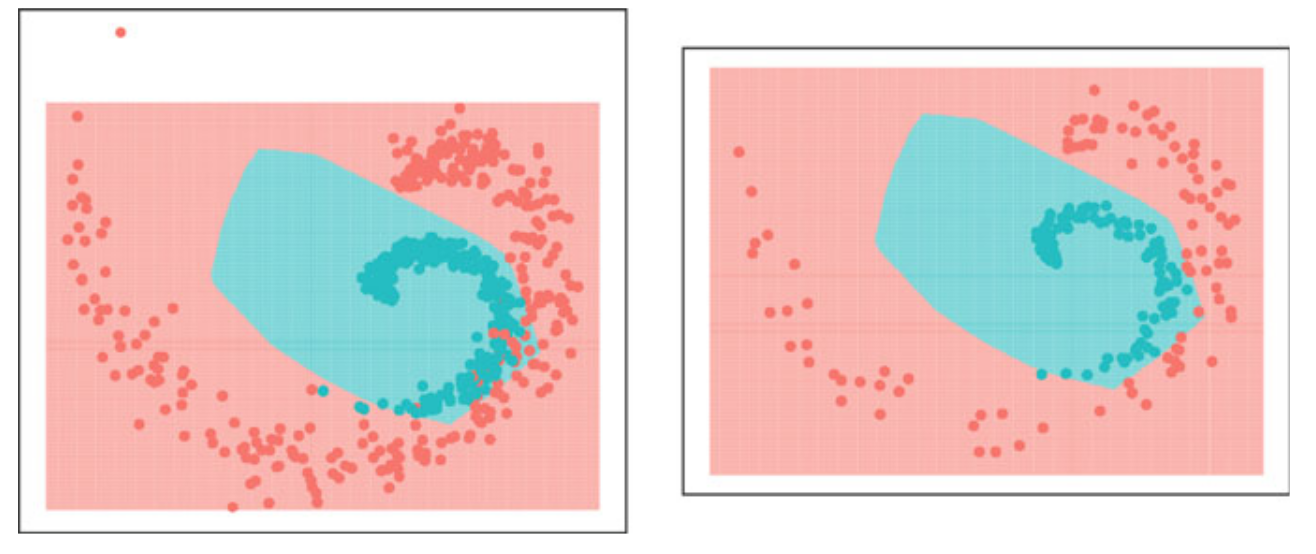
\includegraphics{figure/spiral_planar_data/random.png}}
      \caption{Decision boundary with random initialization ($N\left(0, 1\cdot 10 ^{-4}\right)$) on the training data set (left) and the testing data set (right) (Ghatak, 2019).}
  \end{figure}
      \framebreak
  \begin{figure}
    \centering
      \scalebox{1}{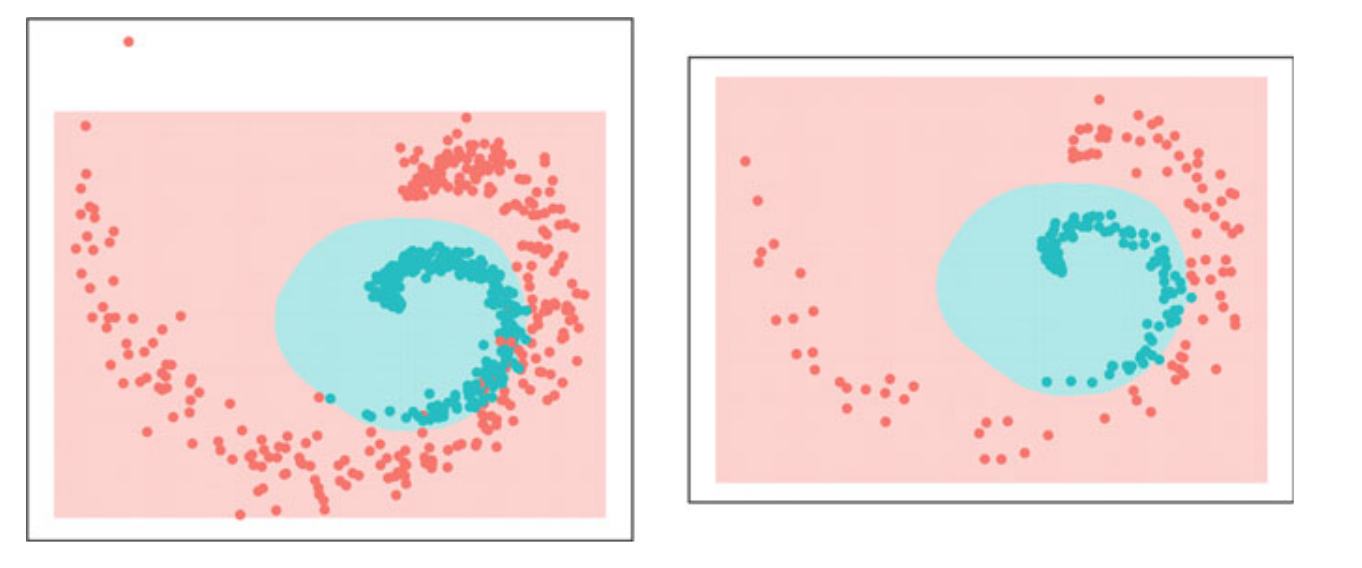
\includegraphics{figure/spiral_planar_data/he.png}}
      \caption{Decision boundary with He initialization on the training data set (left) and the testing data set (right) (Ghatak, 2019).}
  \end{figure}
\end{vbframe}

%%%%%%%%%%%%%%%%%%%%%%%%%%%%%%%%%%%%%%%%%%%%%%%%%%%%%%%%%%%%%%%%%%
\begin{vbframe}{Bias initialization}
  \begin{itemize}
    \item Typically, we set the biases for each unit to heuristically chosen constants. 
    \item Setting the biases to zero is compatible with most weight
initialization schemes as the schemes expect a small bias. 
    \item However, deviations from 0 can be made individually, for example, in order to obtain the right marginal statistics of the output unit or to avoid causing too much saturation at the initialization.
    \item For details see Goodfellow et. al (2016).
  \end{itemize}
\end{vbframe}



%%%%%%%%%%%%%%%%%%%%%%%%%%%%%%%%%%%%%%%%%%%%%%%%%%%%%%%%%%%%%%%%%%
%%%%%%%%%%%%%%%%%%          REFERENCES          %%%%%%%%%%%%%%%%%%
%%%%%%%%%%%%%%%%%%%%%%%%%%%%%%%%%%%%%%%%%%%%%%%%%%%%%%%%%%%%%%%%%%
\begin{vbframe}
\frametitle{References}
\footnotesize{
\begin{thebibliography}{99}
%%%%%%%%%%%%%%%%%%%%%%%%%%%%%%%%%%
% \bibitem[Ian Goodfellow et al., 2016]{1} Ian Goodfellow, Yoshua Bengio and Aaron Courville (2016)
% \newblock Deep Learning
% \newblock \emph{\url{http://www.deeplearningbook.org/}}
% %%%%%%%%%%%%%%%%%%%%%%%%%%%%%%%%%%
% \bibitem[Kaiming He et. al., 2015]{1} Kaiming He, Xiangyu Zhang, Shaoqing Ren, and Jian Sun (2015)
% \newblock Delving Deep into Rectifiers: Surpassing Human-Level Performance on ImageNet Classification. In Proceedings of the 2015 IEEE International Conference on Computer Vision (ICCV) (ICCV '15). IEEE Computer Society, Washington, DC, USA, 1026-1034. 
% \newblock \emph{\url{https://arxiv.org/abs/1502.01852}}
% %%%%%%%%%%%%%%%%%%%%%%%%%%%%%%%%%%
% \bibitem[X. Glorot and Y. Bengio, 2010]{1} Xavier Glorot and Yoshua Bengio  (2010)
% \newblock Understanding the difficulty of training deep feedforward neural networks AISTATS, Volume 9 von JMLR Proceedings, Seite 249-256. JMLR.org
% \newblock \emph{\url{http://proceedings.mlr.press/v9/glorot10a/glorot10a.pdf?hc_location=ufi}}
%%%%%%%%%%%%%%%%%%%%%%%%%%%%%%%%%%%%
\bibitem[(Ghatak, 2019)]{init1} Ghatak, A. (2019). \textit{Deep learning with R}. Springer Singapore. 

\bibitem[Ian Goodfellow et al., 2016]{init2} 
Goodfellow, I., Bengio, Y., \& Courville, A. (2016). \textit{Deep Learning}. MIT Press.
%%%%%%%%%%%%%%%%%%%%%%%%%%%%%%%%%%
\end{thebibliography}
}
\end{vbframe}



%%%%%%%%%%%%%%%%%%%%%%%%%%%%%%%%%%%%%%%%%%%%%%%%%%%%%%%%%%%%%%%%%%
%%%%%%%%%%%%%%%%%%%%%%%%%%%%%%%%%%%%%%%%%%%%%%%%%%%%%%%%%%%%%%%%%%


\begin{frame}{Challenges in Optimization}
 \begin{itemize}
   \item In this section, we summarize several of the most prominent challenges regarding training of deep neural networks.
   \item Traditionally, machine learning ensures that the optimization problem is convex by carefully designing
the objective function and constraints. But for neural networks we are confronted with the general nonconvex case. 
   \item Furthermore, we will see in this section that even convex optimization is not without its complications.
 \end{itemize}
\end{frame}

%%%%%%%%%%%%%%%%%%%%%%%%%%%%%%%%%%%%%%%%%%%%%%%%%%%%%%%%%%%%%%%%%%
\section{Ill-Conditioning}

\begin{frame} {Effects of curvature}

Intuitively, the curvature of a function determines the outcome of a GD step\dots


\vspace*{-0.5cm}
\begin{figure}
\captionsetup{font=footnotesize,labelfont=footnotesize, labelfont = bf}
\begin{center}
	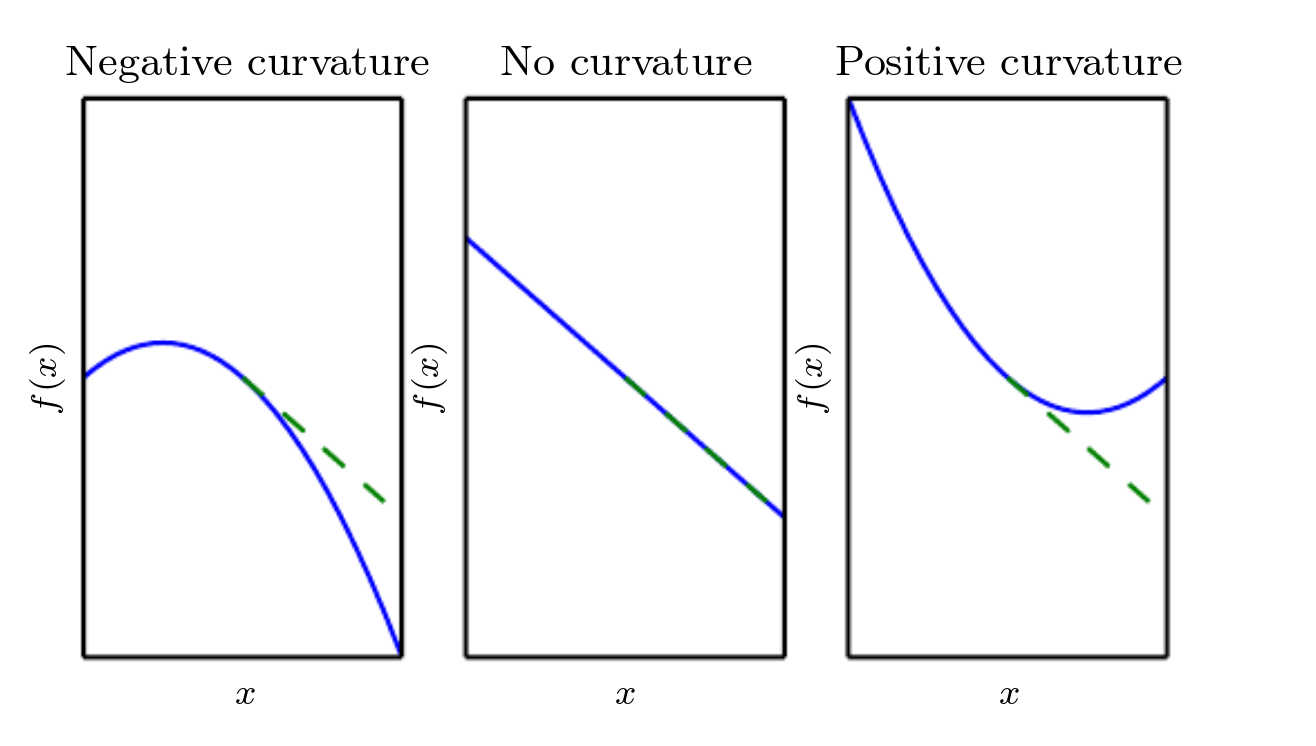
\includegraphics[width=.7\textwidth]{figure/curvature.png}
\end{center}
\tiny{Source: Goodfellow \emph{et al.}, (2016), ch. 4}
\caption{Quadratic objective function $\fx$ with various curvatures.
The dashed line indicates the first order taylor approximation based on the gradient information alone. Left: With negative curvature, the cost function decreases faster than the gradient predicts; Middle: With no curvature, the gradient predicts the decrease correctly; Right: With positive curvature, the function decreases more slowly than expected and begins to increase. }
\end{figure}
\end{frame}

\begin{vbframe}{Second derivative and curvature}

To understand better how the curvature of a function influences the outcome of a gradient descent step, let us recall how curvature is described mathematically: 

\begin{itemize}
  \item The second derivative corresponds to the curvature of the graph of a function. 
  \item The \textbf{Hessian} matrix of a function $\riskt: \mathbb{R}^m \to \mathbb{R}$ is the matrix of second-order partial derivatives
  $$
    H_{ij} = \frac{\partial^2}{\partial \theta_i \partial \theta_j} \riskt.
  $$
\end{itemize}

\framebreak 

\begin{itemize}
  \item The second derivative in a direction $\mathbf{d}$, %of length $1$
   with $\|\mathbf{d}\| = 1$, is given by $\mathbf{d}^\top \!\Hess\,\mathbf{d}$.
  \item What is the direction of the highest curvature (red direction), and what is the direction of the lowest curvature (blue)?
\end{itemize}

\vspace*{-0.5cm}

\begin{figure}
\begin{center}
  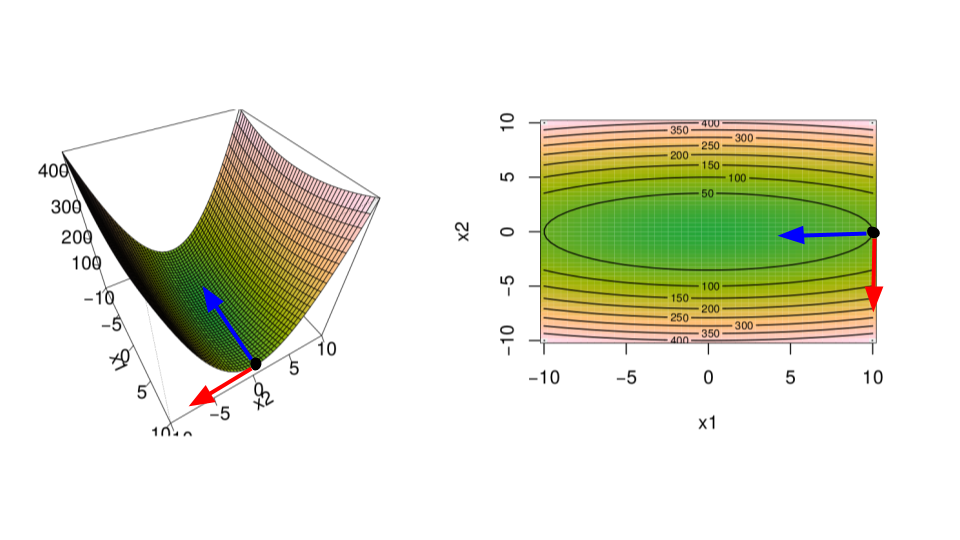
\includegraphics{figure/curvature2.png}
\end{center}
\end{figure}

\framebreak

\begin{itemize}
  \item Since $\Hess$ is real and symmetric (why?), eigendecomposition yields
  $\Hess = \mathbf{V} \mathbf{\diag(\boldsymbol{\lambda})} \mathbf{V}^{-1}$
  with $\mathbf{V}$ and $\boldsymbol{\lambda}$ collecting eigenvectors and eigenvalues, respectively.
  \item It can be shown, that the eigenvector $\textcolor{red}{\bm{v}_{\text{max}}}$ with the max. eigenvalue $\lambda_{\text{max}}$ points into the direction of highest curvature ($\bm{v}_{\text{max}}^\top \bm{H} \bm{v}_{\text{max}} = \lambda_{\text{max}}$), while the eigenvector $\textcolor{blue}{\bm{v}_{\text{min}}}$ with the min. eigenvalue $\lambda_{\text{min}}$ points into the direction of least curvature. 
\end{itemize}

\vspace*{-0.5cm}

\begin{figure}
  \begin{center}
    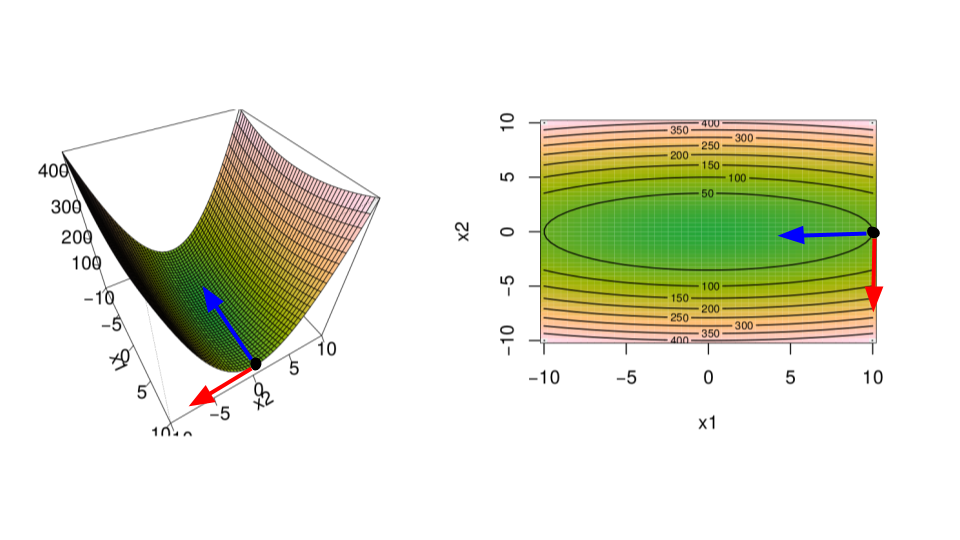
\includegraphics[width=.7\textwidth]{figure/curvature2.png}
  \end{center}
\end{figure}

\framebreak 

\begin{itemize}
  \item At a stationary point $\thetav$, where the gradient is 0, we can examine the eigenvalues of the Hessian to determine whether the $\thetav$ is a local maximum, minimum or saddle point: 
  \vspace{-0.3cm}
  \begin{align*} 
  \quad\forall i: \lambda_i > 0  \, (\Hess \text{ positive definite at $\thetav$}) &\quad\Rightarrow\quad \text{minimum at $\thetav$} \\
  \quad\forall i: \lambda_i < 0 \, (\Hess \text{ negative definite at $\thetav$}) &\quad\Rightarrow\quad \text{maximum at $\thetav$}\\
  \exists\, i: \lambda_i < 0 \land  \exists j: \lambda_j > 0  \,(\Hess \text{ indefinit at $\thetav$}) &\quad\Rightarrow\quad \mbox{saddle point at $\thetav$}
  \end{align*}
\end{itemize}
   \begin{figure}
 \captionsetup{font=footnotesize,labelfont=footnotesize, labelfont = bf}

 \begin{center}
  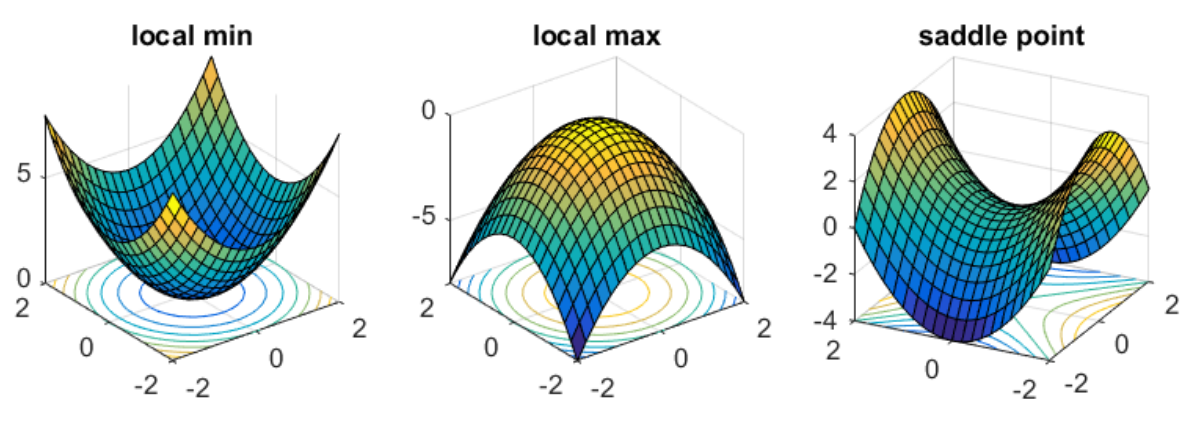
\includegraphics[width=.7\textwidth]{figure/3dim_curvature.png}
 \end{center}
 \tiny{Credit: Rong Ge (2016)}
 \end{figure}

 \end{vbframe}

 \begin{vbframe}{Ill-conditioned Hessian matrix} 


 The condition number of a symmetric matrix $\bm{A}$ is given by the ratio of its min/max eigenvalues $\kappa(\bm{A}) = \frac{|\lambda_{\text{max}}|}{|\lambda_{\text{min}}|}$. A matrix is called ill-conditioned, if the condition number $\kappa(\bm{A})$ is very high. 

 \lz 

 An \textbf{ill-conditioned} Hessian matrix means that the ratio of max. / min. curvature is high, as in the example below: 

\begin{center}
  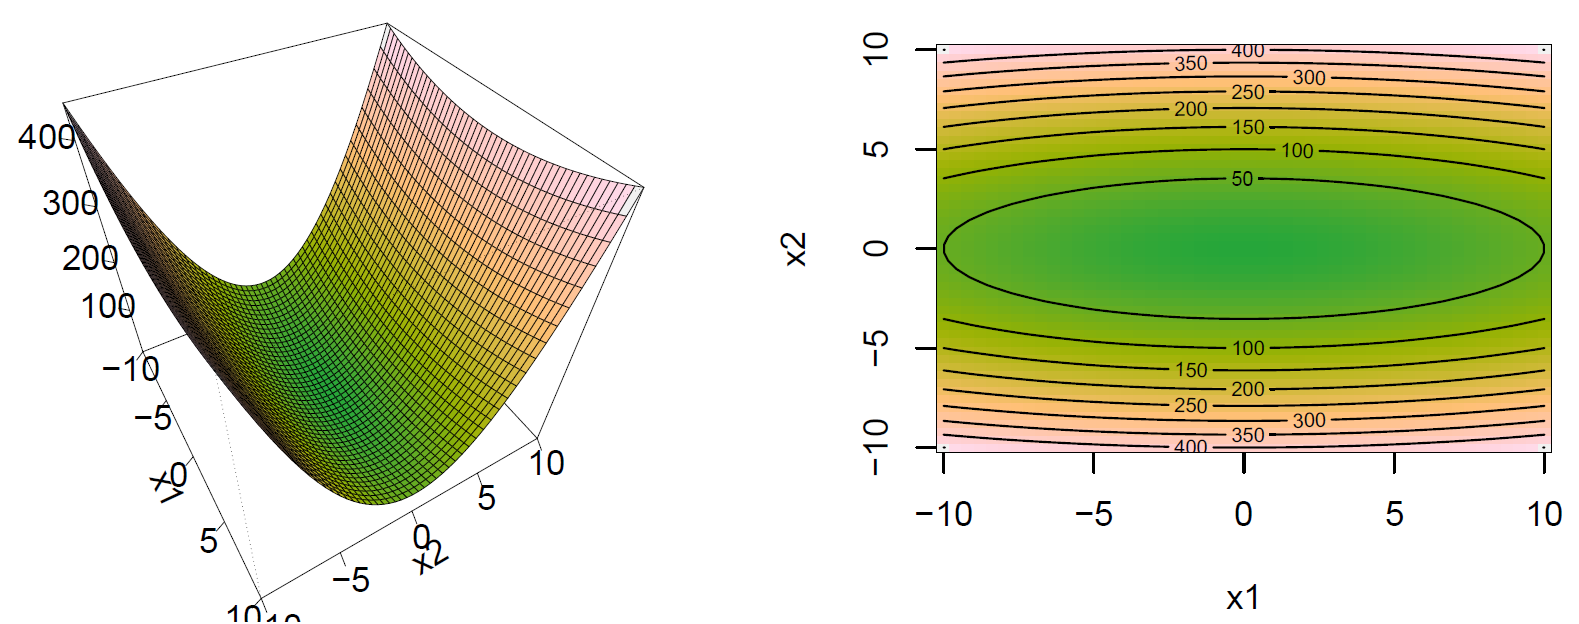
\includegraphics[width=0.7\textwidth]{figure/ill-con.png}
\end{center}


\end{vbframe}

\begin{vbframe}{Curvature and Step-size in GD}

What does it mean for gradient descent if the Hessian is ill-conditioned?

 \begin{itemize}
 \item Let us consider the second-order Taylor approximation as a local approximation of the of $\risk$ around a current point $\boldsymbol{\theta}^0$ (with gradient $\mathbf{g}$)
    \begin{equation*}
    \risk(\boldsymbol{\theta}) \approx T_2f(\thetav, \boldsymbol{\theta}^0) := \risk(\boldsymbol{\theta}^0) + (\boldsymbol{\theta}-\boldsymbol{\theta}^0)^\top \mathbf{g} + \frac{1}{2}(\boldsymbol{\theta}-\boldsymbol{\theta}^0)^\top \!\Hess\, (\boldsymbol{\theta}-\boldsymbol{\theta}^0)
    \end{equation*}
  \item Furthermore, Taylor's theorem states (proof in Koenigsberger (1997), p. 68)
    \begin{equation*}
     \underset{\thetav \rightarrow \boldsymbol{\theta}^0}{\lim} \frac{\risk(\thetav) - T_2f(\thetav, \boldsymbol{\theta}^0)}{||\thetav-\boldsymbol{\theta}^0||^2} = 0
   \end{equation*}

  \framebreak 

  \item One GD step with a learning rate $\alpha$ yields new parameters $\boldsymbol{\theta}^0-\alpha \mathbf{g}$ and a new approximated loss value
   $$
   \risk(\boldsymbol{\theta}^0-\alpha \mathbf{g}) \approx \risk(\boldsymbol{\theta}^0) - \alpha \mathbf{g}^\top\mathbf{g} + \frac{1}{2}	\alpha^2 \mathbf{g}^\top\!\Hess\,\mathbf{g}  \,.
   $$ 
 
 \item Theoretically, if $\mathbf{g}^\top \Hess \mathbf{g}$ is positive, we can solve the equation above for the optimal step size which corresponds to 
 $$
 \alpha^* = \frac{\mathbf{g}^\top \mathbf{g}}{\mathbf{g}^\top \!\Hess\, \mathbf{g}}  \,.
 $$
 
 \framebreak 

 \item Let us assume the gradient $\mathbf{g}$ points into the direction of $\bm{v}_{\text{max}}$ (i.e. the direction of highest curvature), the optimal step size is given by 
  $$
  \alpha^* = \frac{\mathbf{g}^\top \mathbf{g}}{\mathbf{g}^\top \!\Hess\, \mathbf{g}} = \frac{\mathbf{g}^\top \mathbf{g}}{\lambda_{\text{max}} \mathbf{g}^\top   \mathbf{g}} = \frac{1}{\lambda_{\text{max}}}, 
  $$ 
  which is very small. Choosing a too large step-size is bad, as it will make us \enquote{overshoot} the stationary point.
  \item If, on the other hand, $\mathbf{g}$ points into the direction of the lowest curvature, the optimal step size is 
  $$
  \alpha^* = \frac{1}{\lambda_{\text{min}}}, 
  $$
  which corresponds to the largest possible optimal step-size.
  \item We summarize: We want to perform big steps in directions of low curvature, but small steps in directions of high curvature.

  \framebreak 

  \item But what if the gradient does not point into the direction of one of the eigenvectors? 
  \item Let us consider the 2-dimensional case: We can decompose the direction of $\bm{g}$ (black) into the two eigenvectors $\textcolor{red}{\bm{v}_{\text{max}}}$ and $\textcolor{blue}{\bm{v}_{\text{min}}}$
  \item It would be optimal to perform a \textbf{big} step into the direction of the smallest curvature $\textcolor{blue}{\bm{v}_{\text{min}}}$, but a \textbf{small} step into the direction of $\textcolor{red}{\bm{v}_{\text{max}}}$, but the gradient points into a completely different direction. 
  \end{itemize}

  \vspace*{-0.4cm}

  \begin{figure}
    \begin{center}
      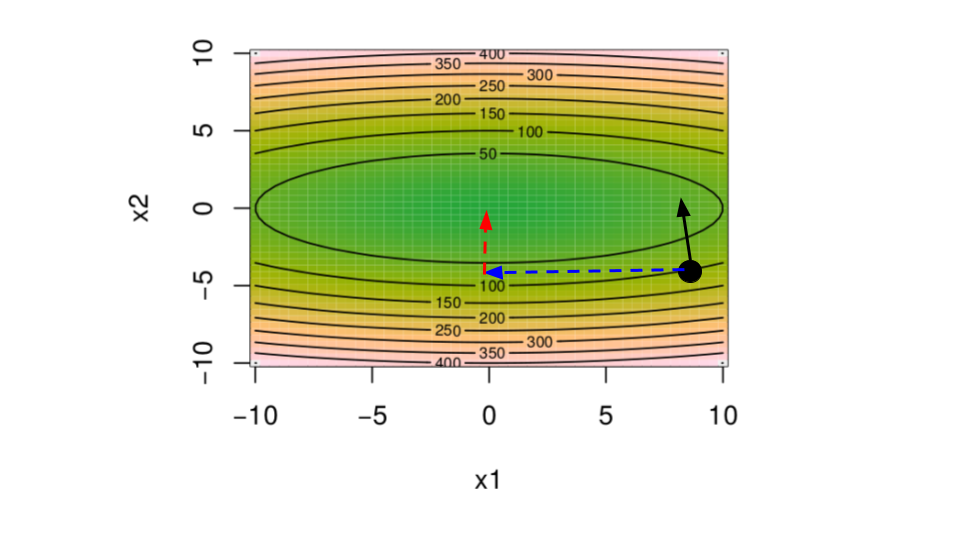
\includegraphics[width=.7\textwidth]{figure/curvature3.png}
    \end{center}
  \end{figure}

\end{vbframe}

% \begin{frame} {Effects of curvature}
% \begin{itemize}
% \item The second-order Taylor approximation (with gradient $\mathbf{g}$) around current point $\boldsymbol{\theta}^0$ is
% \begin{equation*}
% \risk(\boldsymbol{\theta}) = \risk(\boldsymbol{\theta}^0) + (\boldsymbol{\theta}-\boldsymbol{\theta}^0)^\top \mathbf{g} + \frac{1}{2}(\boldsymbol{\theta}-\boldsymbol{\theta}^0)^\top \!\Hess\, (\boldsymbol{\theta}-\boldsymbol{\theta}^0)
% \end{equation*}
% \item SGD with learning rate $\alpha$ yields new parameters $\boldsymbol{\theta}^0-\alpha g$ and new loss value
% $$
% \risk(\boldsymbol{\theta}^0-\alpha \mathbf{g}) = \risk(\boldsymbol{\theta}^0) - \alpha \mathbf{g}^\top\mathbf{g} + \frac{1}{2}	\alpha^2 \mathbf{g}^\top\!\Hess\,\mathbf{g}  \,.
% $$
% \item When $g^\top H g$ is to large, we might get $\risk(\boldsymbol{\theta}^0-\alpha \mathbf{g}) > \risk(\boldsymbol{\theta}^0)$.
% \item If $\mathbf{g}^\top \Hess \mathbf{g}$ is positive, optimal step size is
% $$
% \alpha^* = \frac{\mathbf{g}^\top \mathbf{g}}{\mathbf{g}^\top \!\Hess\, \mathbf{g}} \ge \frac{1}{\lambda_{\text{max}}}  \,.
% $$
% \end{itemize}
% \end{frame}

\begin{vbframe} {Ill-conditioning}


\begin{itemize}
  %   \item The new risk after a \textbf{gradient descent} step is 
  %   $$
  %   \risk(\boldsymbol{\theta}^0-\alpha \mathbf{g}) \approx \risk(\boldsymbol{\theta}^0) \underbrace{- \alpha \mathbf{g}^\top\mathbf{g} + \frac{1}{2}	\alpha^2 \mathbf{g}^\top\!\Hess\,\mathbf{g}}_{:=\nu}  \,.
  %   $$ 
  % The term  $\nu$ is added to the risk $\risk$ in each gradient descent step. 
  %   \item Ill-conditioning of the Hessian matrix $\Hess$ becomes a problem, when $$\frac{1}{2}	\alpha^2 \mathbf{g}^\top\!\Hess\,\mathbf{g}^\top > \alpha \mathbf{g}^\top\mathbf{g}$$
  %   \item Ill-conditioning occurrs, if the second derivatives for a specific point differ a lot. This can be measured by the condition number. A condition number of 5, for example, means that the direction of the highest curvature has five times more curvature than the direction of the least  curvature. 

  % \framebreak 
  \item GD is unaware of large differences in curvature, and can only walk into the direction of the gradient.  
  \item Choosing a too large step-size will then cause the descent direction change frequently (\enquote{jumping around}).
  \item $\alpha$ needs to be small enough, which results in a low progress.
  
  \framebreak
  
  \item This effect is more severe, if a Hessian has a poor condition number, i.e. the ratio between lowest and highest curvature is large; gradient descent will perform poorly. 
  \begin{figure}
  \captionsetup{font=footnotesize,labelfont=footnotesize, labelfont = bf}
  \begin{center}
  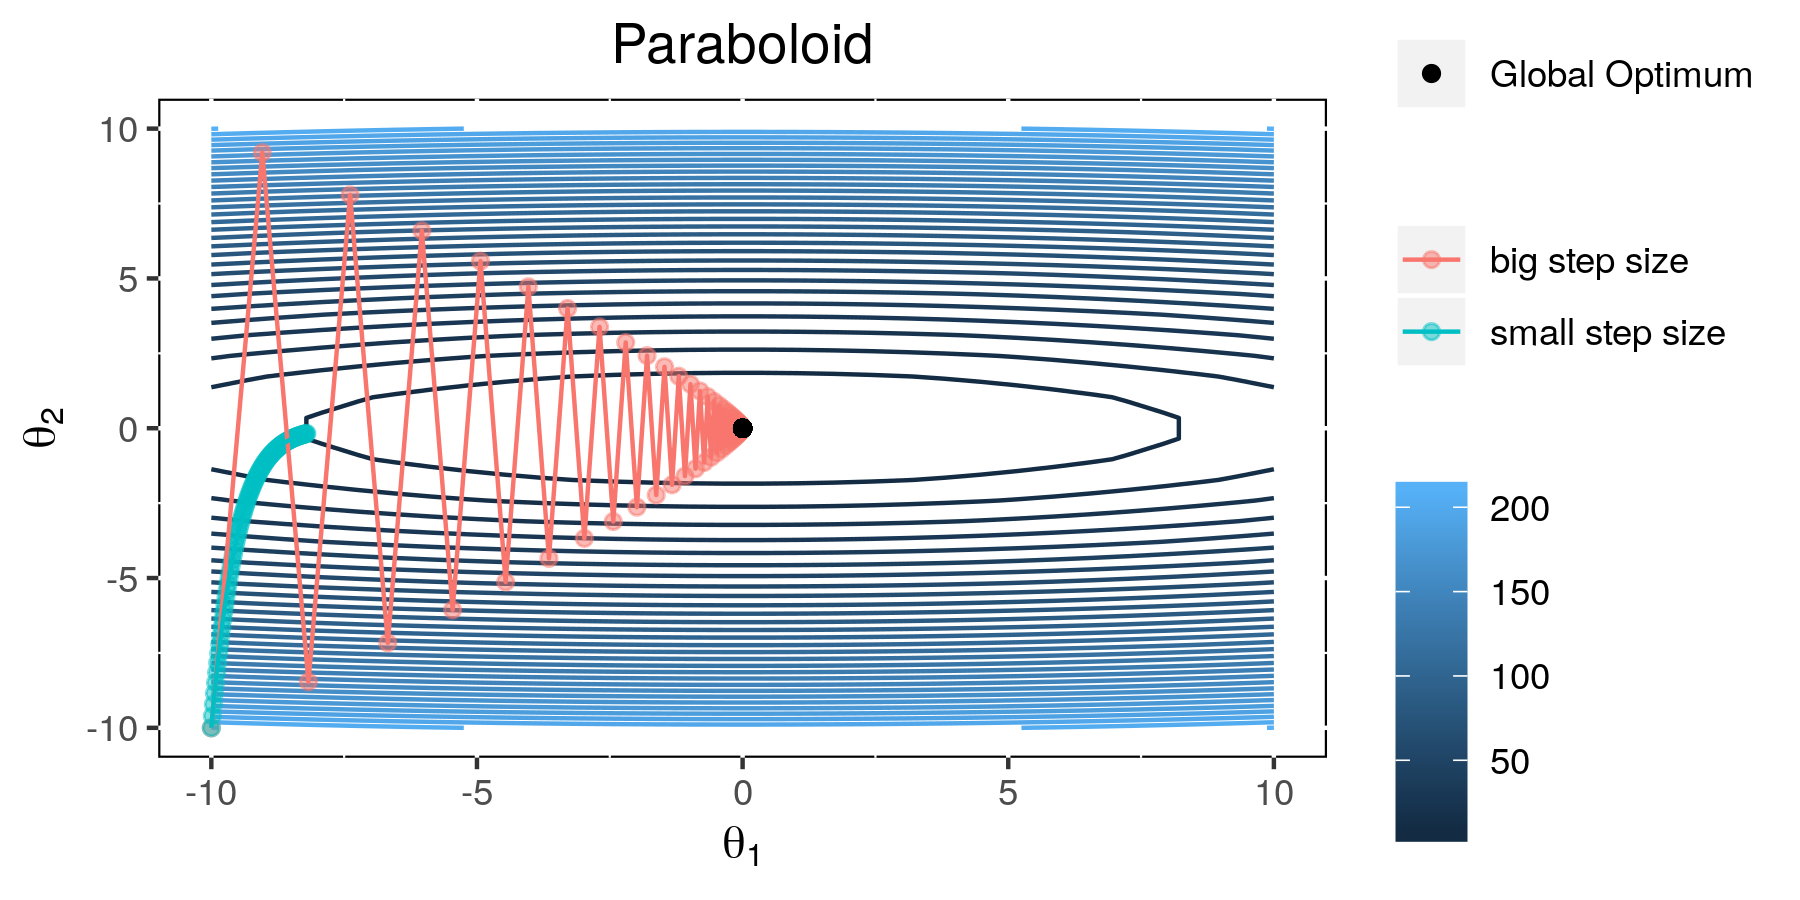
\includegraphics[width=0.7\textwidth]{figure/big_small_stepsize.png}
  \end{center}
  \caption{The contour lines show a quadratic risk function with a poorly conditioned Hessian matrix. The plot shows the progress of gradient descent with a small step-size vs. larger step-size. In both cases, convergence to the global optimum is rather slow. }
  \end{figure}

  \item In the worst case, ill-conditioning of the Hessian matrix and a too big step-size will cause the risk to increase

    $$
   \risk(\boldsymbol{\theta}^0-\alpha \mathbf{g}) \approx \risk(\boldsymbol{\theta}^0) - \alpha \mathbf{g}^\top\mathbf{g} + \frac{1}{2} \alpha^2 \mathbf{g}^\top\!\Hess\,\mathbf{g}  \,,
   $$ 
   which happens if 
   $$
    \frac{1}{2} \alpha^2 \mathbf{g}^\top\!\Hess\,\mathbf{g} > \alpha \mathbf{g}^\top\mathbf{g}.
   $$
    \item To determine whether ill-conditioning is detrimental to the training, the squared gradient norm $\mathbf{g}^\top \mathbf{g}$ and the risk %and the term $\mathbf{g}^\top\Hess\mathbf{g}$ 
    can be monitored.

    \begin{figure}
      \captionsetup{font=footnotesize,labelfont=footnotesize, labelfont = bf}
    \centering
      \scalebox{0.8}{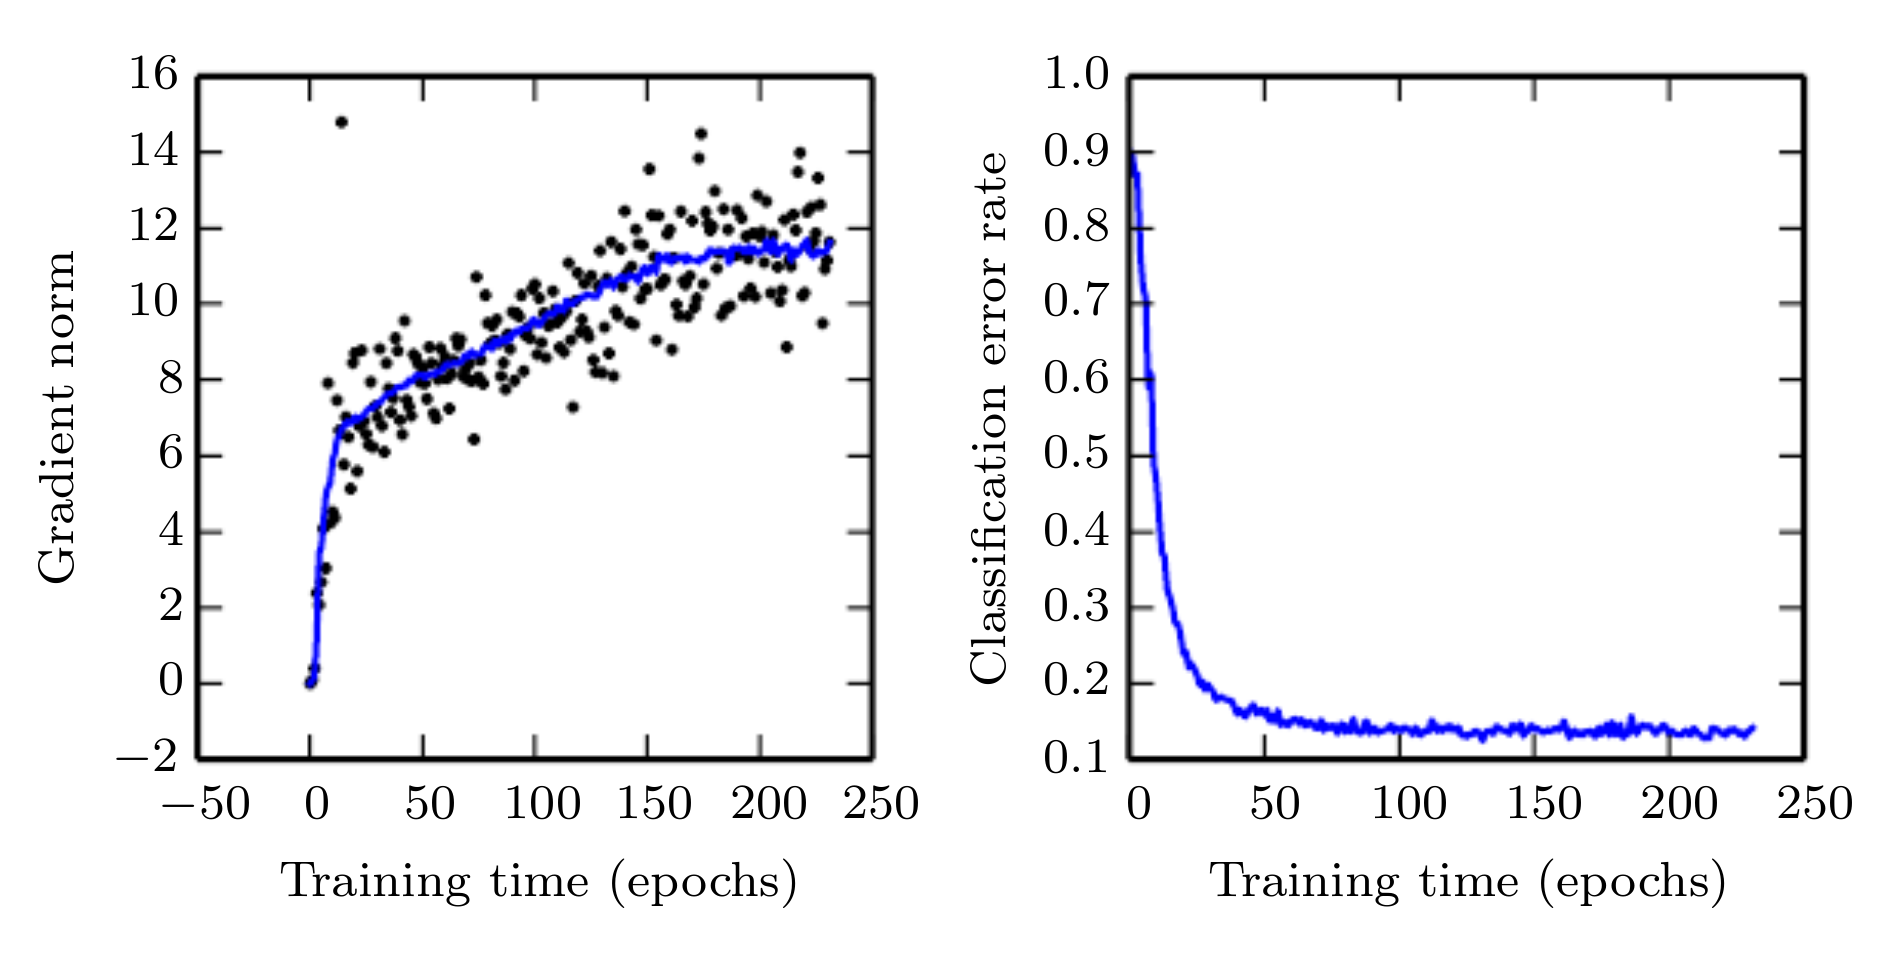
\includegraphics{figure/no_critical.png}}
      \tiny{\\Source: Goodfellow, ch. 6}
    \end{figure}

    \vspace*{-0.1cm}

    \item Gradient norms \textbf{increase} over time, showing that the training process is not converging to a stationary point $\mathbf{g} = 0$. 
    \item At the same time, we observe that the risk is approx. constant, but the gradient norm increases
    \vspace*{-0.2cm}
    $$
      \underbrace{\risk(\boldsymbol{\theta}^0-\alpha \mathbf{g})}_{\text{approx. constant}} \approx \risk(\boldsymbol{\theta}^0) - \underbrace{\alpha \mathbf{g}^\top\mathbf{g}}_{\text{increase}}+ \frac{1}{2}  \underbrace{\alpha^2 \mathbf{g}^\top\!\Hess\,\mathbf{g}}_{\to \text{increase}}  \,. 
     $$ 
  \end{itemize}
\end{vbframe}

%%%%%%%%%%%%%%%%%%%%%%%%%%%%%%%%%%%%%%%%%%%%%%%%%%%%%%%%%%%%%%%
\section{Local Minima}

\begin{vbframe}{Unimodal vs. Multimodal loss surfaces}
  \begin{figure}
  \centering
    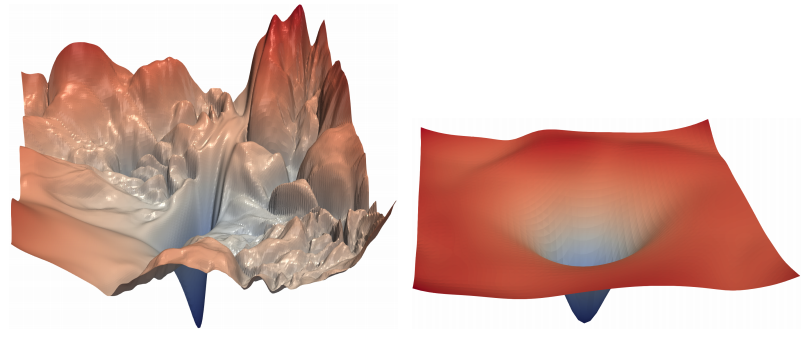
\includegraphics[width=12cm]{figure/difficult_vs_easy.png}
    \caption{Left: Multimodal loss surface with saddle points; Right: (Nearly) unimodal loss surface (Hao Li et al. (2017))}
  \end{figure}
\end{vbframe}

%%%%%%%%%%%%%%%%%%%%%%%%%%%%%%%%%%%%%%%%%%%%%%%%%%%%%%%%%%%%%%%%%%

\begin{vbframe}{Multimodal function}
Potential snippet from a loss surface of a deep neural network with many local minima:

\begin{center}
  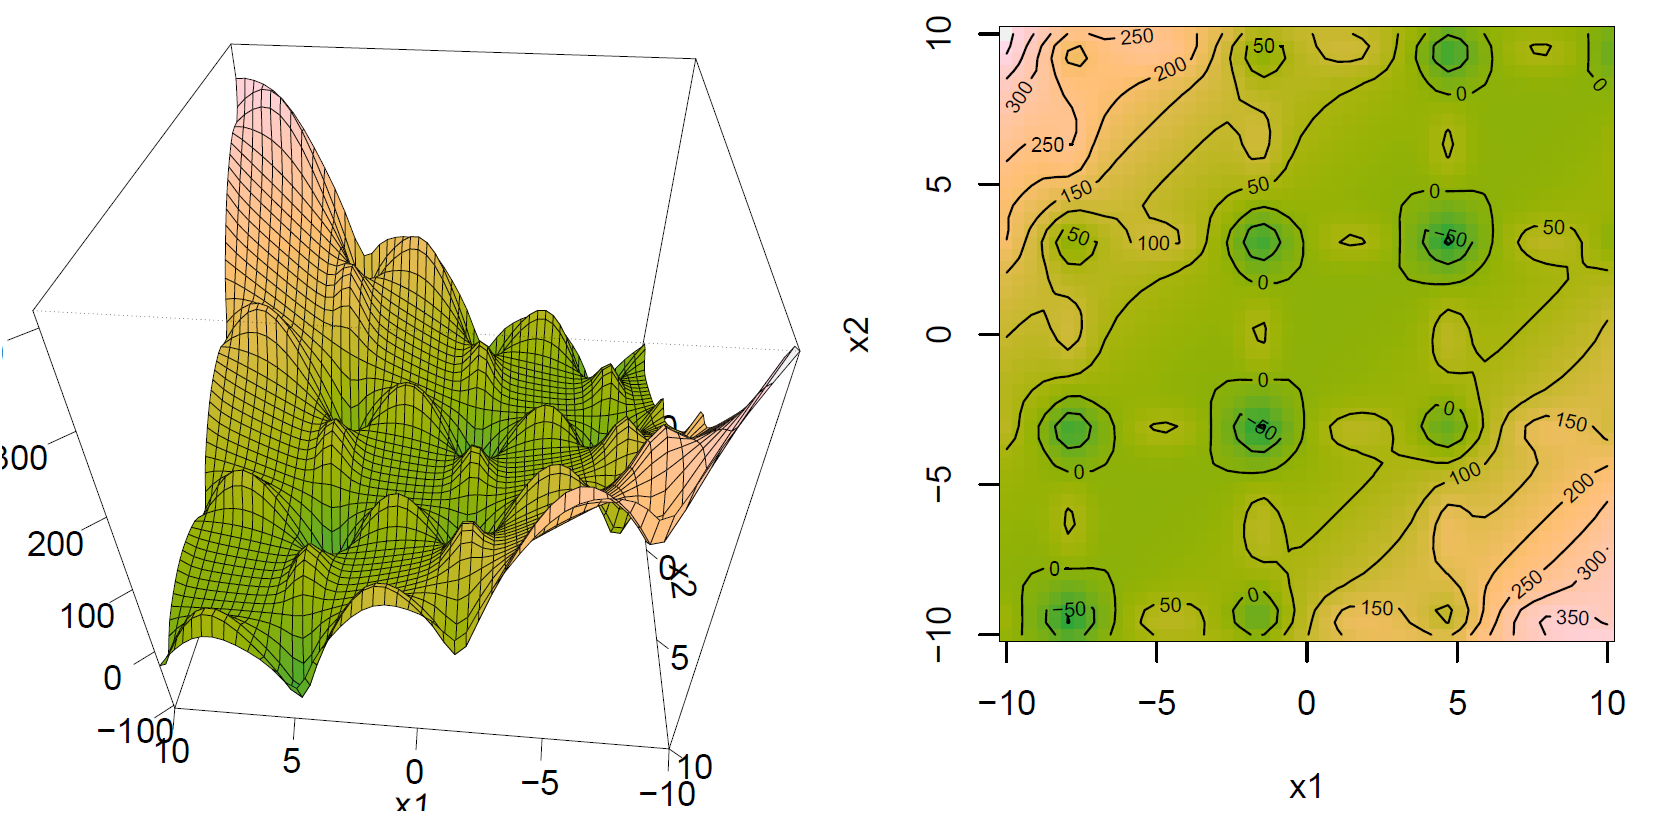
\includegraphics[width=.9\textwidth]{figure/multimodal.png}
\end{center}

\end{vbframe}

\begin{frame} {Only locally optimal moves}
  \begin{itemize}
  \small{
    \item If the training algorithm makes only \textit{locally} optimal moves (as in gradient descent), it may move away from regions of \textit{much} lower cost.
      \begin{figure}
    \centering
      \scalebox{0.65}{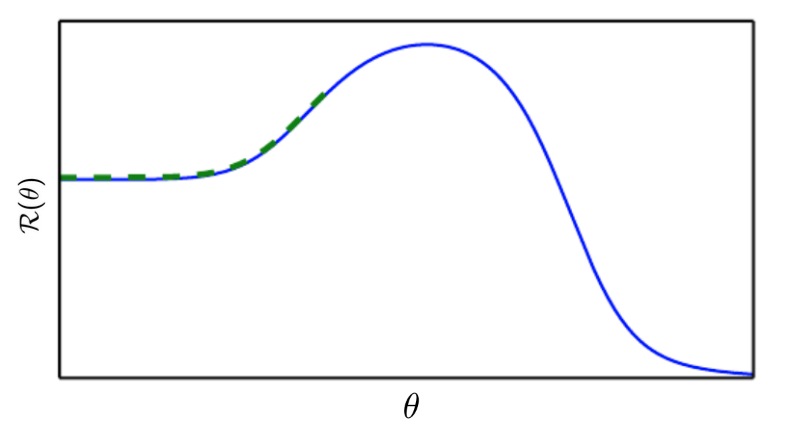
\includegraphics{figure/local_hill.png}}
      \tiny{\\Source: Goodfellow, Ch. 8}
    \end{figure}
    \item In the figure above, initializing the parameter on the "wrong" side of the hill will result in suboptimal performance.
    \item In higher dimensions, however, it may be possible for gradient descent to go around the hill but such a trajectory might be very long and result in excessive training time.}
  \end{itemize}
\end{frame}

\begin{vbframe} {Local minima}
   Weight space symmetry:
   \begin{itemize}
       \item If we swap incoming weight vectors for neuron $i$ and $j$
       and do the same for the outcoming weights,
       modelled function stays unchanged.
        \begin{itemize}
           \item[$\Rightarrow$] with $n$ hidden units and one hidden layer
           there are $n!$ networks with the same empirical risk
        \end{itemize}
       \item If we multiply incoming weights of a ReLU neuron with $\beta$
       and outcoming with $1/\beta$ the modelled function stays unchanged.
      \end{itemize}
  $\Rightarrow$ The empirical risk of a NN can have very many
          minima with equivalent empirical risk.

\framebreak 

    \begin{itemize}
     \item In practice only local minima with a high value compared to the global minimium are problematic.
    \begin{figure}
     \begin{center}
     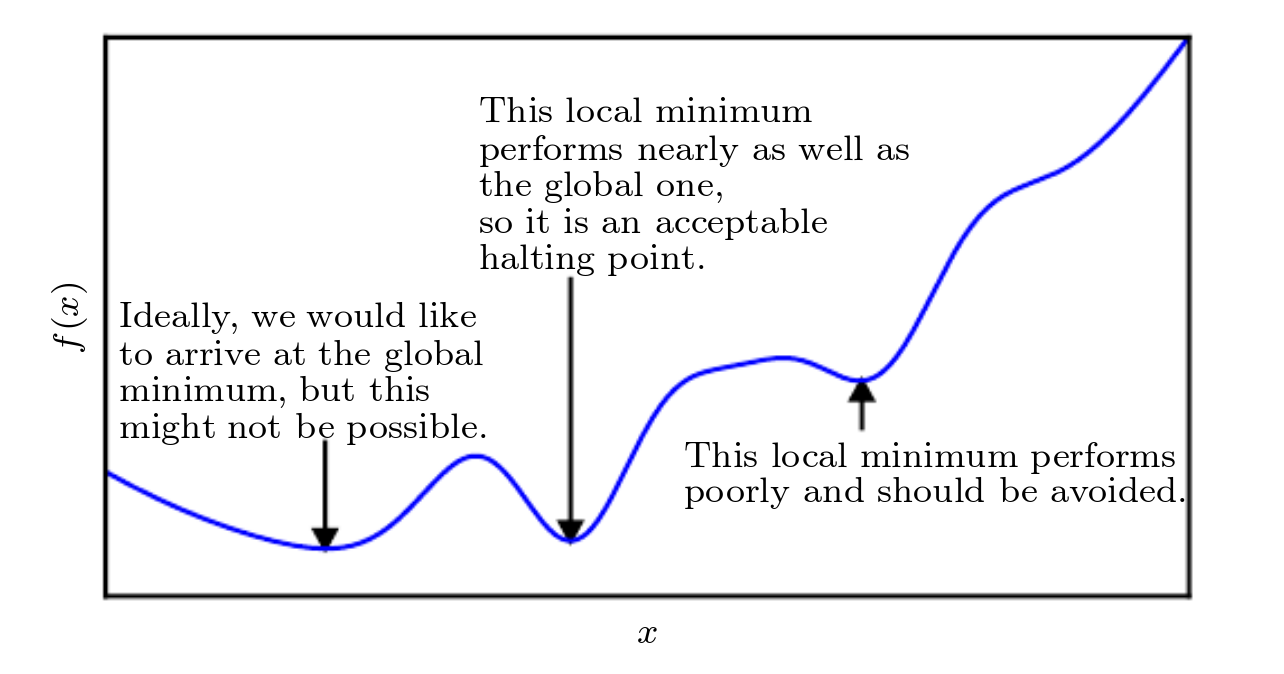
\includegraphics[width=.6\textwidth]{figure/minima.png}
     \end{center}
    \tiny{Source: Goodfellow, Ch. 4}
    \end{figure}
     \item Current literature suspects that most local minima have low empirical risk.
\end{itemize}
\end{vbframe}

%%%%%%%%%%%%%%%%%%%%%%%%%%%%%%%%%%%%%%%%%%%%%%%%%%%%%%%%%%%%%%%%%%
\section{Saddle Points}
\begin{vbframe}{Saddle Points}
  \begin{itemize}
    \item In optimization we look for areas with zero gradient.
    \item A variant of zero gradient areas are saddle points.
    \item For the empirical risk $\risk$ of a neural network, the expected ratio of the number of saddle points to local minima typically grows exponentially with $m$ 
    $$\risk: \mathbb{R}^m \rightarrow \mathbb{R}$$ 
    In other words: Networks with more parameters (deeper networks or larger layers) exhibit a lot more saddle points than local minima.
     \item Why is that?
    \item The Hessian at a local minimum has only positive eigenvalues. At a saddle point it is a mixture of positive and negative eigenvalues.
    
\framebreak
    
    \item Imagine the sign of each eigenvalue is generated by coin flipping:
    \begin{itemize}
      \item In a single dimension, it is easy to obtain a local minimum (e.g. \enquote{head} means positive eigenvalue).
      \item In an $m$-dimensional space, it is exponentially unlikely that all $m$ coin tosses will be head.
    \end{itemize}
    \item A property of many random functions is that eigenvalues of the Hessian become more likely to be positive in regions of lower cost.
    \item For the coin flipping example, this means we are more likely to have heads $m$ times if we are at a critical point with low cost.
    \item That means in particular that local minima are much more likely to have low cost than high cost and critical points with high cost are far more likely to be saddle points.
    \item See Dauphin et al. (2014) for a more detailed investigation.
  \end{itemize}
\end{vbframe}

\begin{vbframe}{Saddle Points: Example}
  \begin{center}
    $f(x_1, x_2) = x_1^2 - x_2^2$
  \end{center}
  \begin{figure}
    \centering
    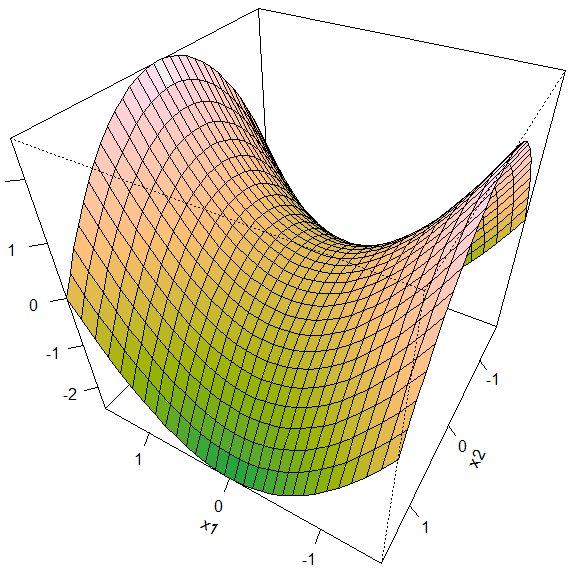
\includegraphics[width=4cm]{figure/saddlepoint.png}
  \end{figure} 
  \begin{itemize}
    \item Along $x_1$, the function curves upwards (eigenvector of the Hessian with positive eigenvalue). Along $x_2$, the function curves downwards (eigenvector of the Hessian with negative eigenvalue).
  \end{itemize}
\end{vbframe}

\begin{vbframe}{Saddle Points}
  \begin{itemize}
    \item So how do saddle points impair optimization?
    \item First-order algorithms that use only gradient information \textbf{might} get stuck in saddle points.
    \item Second-order algorithms experience even greater problems when dealing with saddle points. Newtons method for example actively searches for a region with zero gradient. That might be another reason why second-order methods have not succeeded in replacing gradient descent for neural network training. 
  \end{itemize}
\end{vbframe}

%%%%%%%%%%%%%%%%%%%%%%%%%%%%%%%%%%%%%%%%%%%%%%%%%%%%%%%%%%%

\frame{

\frametitle{Example: Saddle point with GD}

  \center
  \only<1>{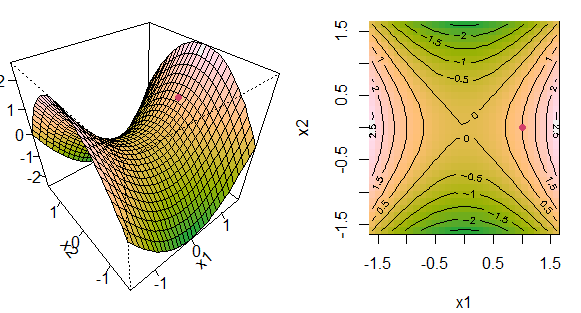
\includegraphics[width=9cm]{figure/opt1.png}}%
  \only<2>{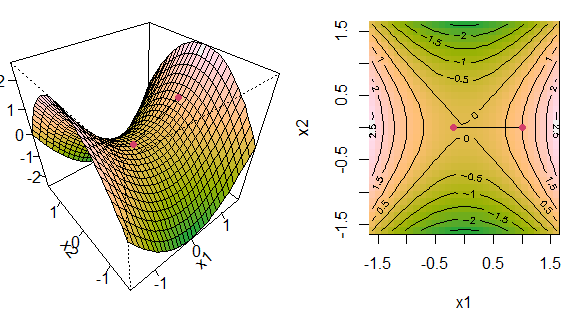
\includegraphics[width=9cm]{figure/opt2.png}}%
  \only<3>{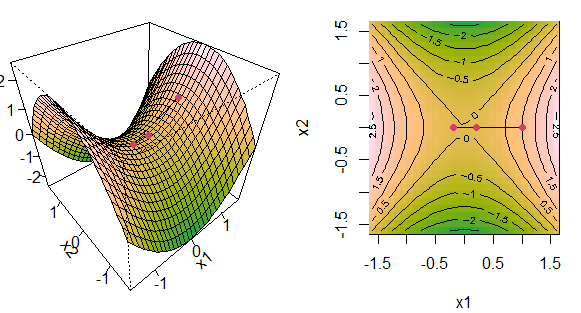
\includegraphics[width=9cm]{figure/opt3.png}}%
  \only<4>{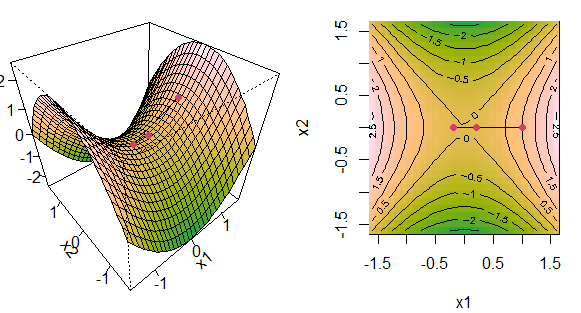
\includegraphics[width=9cm]{figure/opt10.png}}%
  
  \begin{itemize}

    \only<1>{\item[] \small{Red dot: Starting location}}
    \only<2>{\item[] \small{First step...}}
    \only<3>{\item[] \small{...second step...}}
    \only<4>{\item[] \small{...tenth step got stuck and cannot escape the saddle point!}}
    
  \end{itemize}

}

\section{Cliffs and Exploding Gradients}
\begin{vbframe}{Cliffs and exploding gradients}
  \begin{itemize}
    \item As a result from the multiplication of several parameters, the emprirical risk for highly nonlinear deep neural networks often contain sharp nonlinearities.
      \begin{itemize}
        \item That may result in very high derivatives in some places.
        \item As the parameters get close to such cliff regions, a gradient descent update can catapult the parameters very far.
        \item Such an occurrence can lead to losing most of the optimization work that had been done.
      \end{itemize}
    \item However, serious consequences can be easily avoided using a technique called \textbf{gradient
clipping}.
    \item The gradient does not specify the optimal step size, but only the optimal direction
within an infinitesimal region.
\framebreak 
    \item Gradient clipping simply caps the step size to be small enough that it is less likely to go outside the region where the gradient indicates the direction of steepest descent.
    \item We simply \enquote{prune} the norm of the gradient at some threshold $h$:
    $$\text{if  } ||\nabla \thetav|| > \text h: \nabla \thetav \leftarrow \frac{h}{||\nabla \thetav||} \nabla \thetav $$
  \end{itemize}
\end{vbframe}

%%%%%%%%%%%%%%%%%%%%%%%%%%%%%%%%%%%%%%%%%%%%%%%%%%%%%%

\begin{vbframe}{Example: cliffs and exploding gradients}
  \begin{figure}
  \centering
    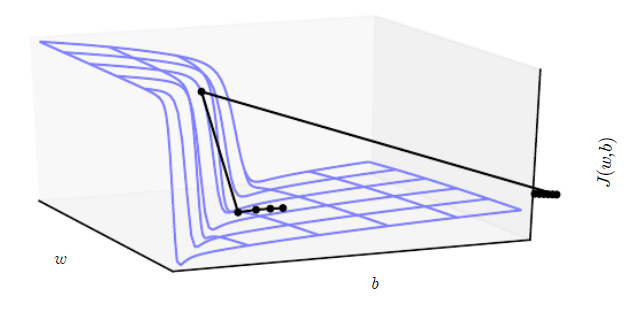
\includegraphics[width=8cm]{figure/cliff2.png}
    \caption{\enquote{The objective function for highly nonlinear deep neural networks or for
recurrent neural networks often contains sharp nonlinearities in parameter space resulting
from the multiplication of several parameters. These nonlinearities give rise to very
high derivatives in some places. When the parameters get close to such a cliff region, a
gradient descent update can catapult the parameters very far, possibly losing most of the
optimization work that had been done} (Goodfellow et al. (2016)).}
  \end{figure}
\end{vbframe}

%%%%%%%%%%%%%%%%%%%%%%%%%%%%%%%%%%%%%%%%%%%%%%%%%%%%%%%%%%%%%%%%%%
%%%%%%%%%%%%%%%%%%          REFERENCES          %%%%%%%%%%%%%%%%%%
%%%%%%%%%%%%%%%%%%%%%%%%%%%%%%%%%%%%%%%%%%%%%%%%%%%%%%%%%%%%%%%%%%
\begin{vbframe}
\frametitle{References}
\footnotesize{
\begin{thebibliography}{99}
%%%%%%%%%%%%%%%%%%%%%%%%%%%%%%%%%%
\bibitem[Ian Goodfellow et al., 2016]{chal1} Ian Goodfellow, Yoshua Bengio and Aaron Courville (2016)
\newblock Deep Learning
\newblock \emph{\url{http://www.deeplearningbook.org/}}
%%%%%%%%%%%%%%%%%%%%%%%%%%%%%%%%%%
\bibitem[Yann Dauphin et al., 2014]{chal2} Yann Dauphin, Razvan Pascanu, {\c{C}}aglar G{\"{u}}l{\c{c}}ehre, Kyunghyun Cho, Surya Ganguli, Yoshua Bengio (2014)
\newblock Identifying and attacking the saddle point problem in high-dimensional non-convex optimization
\newblock \emph{\url{https://arxiv.org/abs/1406.2572}}
%%%%%%%%%%%%%%%%%%%%%%%%%%%%%%%%%%
\bibitem[Hao Li et al., 2017]{chal3} Hao Li, Zheng Xu, Gavin Taylor, Christoph Studer, Tom Goldstein (2017)
\newblock Visualizing the Loss Landscape of Neural Nets
\newblock \emph{\url{https://arxiv.org/abs/1712.09913}}
%%%%%%%%%%%%%%%%%%%%%%%%%%%%%%%%%%
\bibitem[Koenigsberger, 1997]{chal4} Konrad Koenigsberger (1997)
\newblock Analysis 2, Springer
%%%%%%%%%%%%%%%%%%%%%%%%%%%%%%%%%
\bibitem[Ge (2016)]{chal5} Rong Ge (2016)
\newblock Escaping from Saddle Points
\newblock \emph{\url{http://www.offconvex.org/2016/03/22/saddlepoints/}}

\end{thebibliography}
}
\end{vbframe}

\begin{vbframe}{License \& Attribution}
\begin{itemize}
\item This deck is adapted from \textbf{Introduction to Deep Learning (I2DL)},
Prof.\ Dr.\ Bernd Bischl, Statistical Learning and Data Science (SLDS),
LMU Munich. \url{https://github.com/slds-lmu/lecture_i2dl}
\item Licensed \textbf{CC BY 4.0}: \url{https://creativecommons.org/licenses/by/4.0/}
\item Content has been merged, reordered, and consolidated from the original
per-topic decks into this single session deck; not used verbatim.
\end{itemize}
\end{vbframe}

\endlecture
\end{document}
